%----------------------------------------------------------------------------------------
%	PACKAGES & THEMES
%----------------------------------------------------------------------------------------

\documentclass[8pt]{beamer}

\usepackage{etex}
\mode<presentation> {
\usetheme{Vilanova}
}

\usepackage[english]{babel}
\usepackage[utf8]{inputenc}
\usepackage{array}
\usepackage{graphicx}
\usepackage{booktabs}
\usepackage{amsmath,amssymb,amsthm}
\usepackage{xcolor}
\usepackage{tikz}
\usetikzlibrary{arrows}
\usepackage{pifont}
\usepackage{listings,color}

\definecolor{listcomment}{rgb}{0.0,0.5,0.0}
\definecolor{listkeyword}{rgb}{0.0,0.0,0.5}
\definecolor{listnumbers}{gray}{0.65}
\definecolor{listlightgray}{gray}{0.955}
\definecolor{listwhite}{gray}{1.0}

\AtBeginSection[]
{
\addtocounter{framenumber}{-1}
\begin{frame}
\frametitle{Outline}
\tableofcontents[currentsection]
\end{frame}}

%----------------------------------------------------------------------------------------
%	TITLE PAGE
%----------------------------------------------------------------------------------------
\title{Orfeo ToolBox}
\subtitle{Open source processing of remote sensing images (updated for 6.2)}
\author{OTB Team}
\date{}

\pgfdeclareimage[height=96mm,width=128mm]{background}{images/fondsClairSansLogo}
\pgfdeclareimage[height=0.2cm]{cc}{images/CC-licence.png}
\setbeamertemplate{background}{\pgfuseimage{background}}
\pgfdeclareimage[height=0.6cm]{logoIncrust}{images/logoIncrust}
\pgfdeclareimage[height=0.6cm]{OSGeo_logo}{images/OSGeo_logo}
\logo{
\begin{tabular}{p{0.22\textwidth}p{0.58\textwidth}p{0.1\textwidth}p{0.1\textwidth}}
\href{http://www.osgeo.org}{\pgfuseimage{OSGeo_logo}}
& \vspace{-0.03\textwidth} \scriptsize{} % date and event here
& \href{http://creativecommons.org/licenses/by-sa/3.0/}{\pgfuseimage{cc}} & \href{http://www.orfeo-toolbox.org}{\pgfuseimage{logoIncrust}}\\
\end{tabular}
}

\titlegraphic{\vspace*{-5em}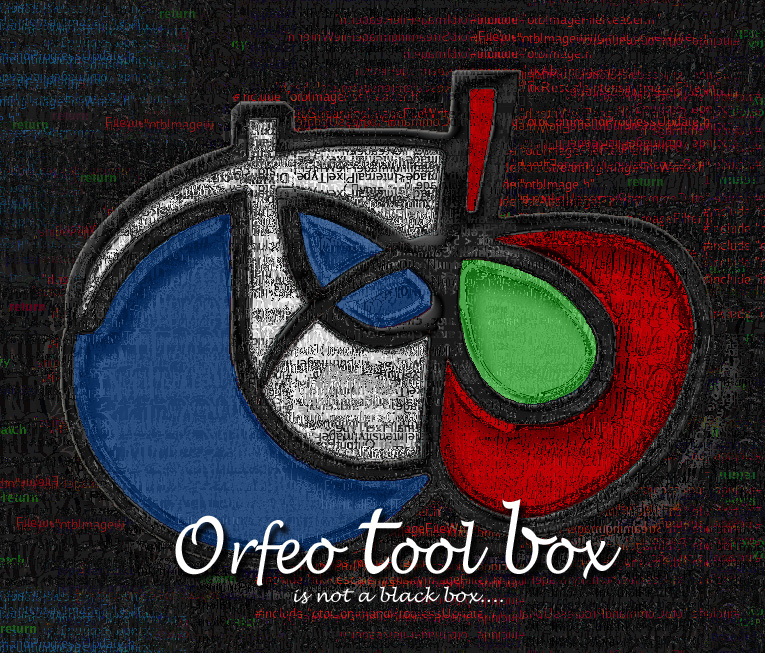
\includegraphics[width=.5\textwidth]{images/LOGOTB_blackbox.png}}

\begin{document}
\begin{frame}
\titlepage
\end{frame}

\mode<all>
\section*{Introduction}

\begin{frame}
\frametitle{Things to know about OTB\ldots}
\begin{block}{Orfeo ToolBox is:}
\begin{itemize}
\item An \textbf{image processing library} for remote sensing
\item \textbf{Free and open source software} under Apache v2.0 license (since 6.0, formerly CeCILL-v2)
\item \textbf{Funded and developed by CNES} (French Space Agency) in the frame
  the development of the Pléiades satellite (and beyond)
\item A project of OSGeo since 2017
\item Used at CNES, ESA (European Space Agency), mission exploitation platforms,
  remote sensing labs, teaching\ldots
\item Written in \textbf{C++} on top of \href{www.itk.org}{ITK} (medical image
  processing)
\item Built on the shoulders of giants (GDAL, OSSIM, OpenCV\ldots)
\item \textbf{Big Data} capable, thanks to built-in streaming and multithreading
\end{itemize}
\end{block}

\begin{center}
{\huge\textcolor{red}{\href{http://www.orfeo-toolbox.org}{orfeo-toolbox.org}}}
\end{center}

\end{frame}

\begin{frame}
\frametitle{Why open source?}

\begin{block}{Maximum reach}
OTB is dedicated to every user of satellite images. Its wide
dissemination contributes to the missions success (Pléiades, Sentinels\ldots)
\end{block}

\begin{block}{Quality and efficiency}
OTB covers a vast panel of applications and thematic fields. Openness should:
\begin{itemize}
\item Facilitate appropriation and validation for users
\item Encourage contributions and bug reports
\item Available on multiple platforms
\item ``The Cathedral \& the
  Bazaar''\footnote{\url{http://www.catb.org/esr/writings/cathedral-bazaar/}}: the more widely available the source code is for public testing
  experimentation, the more rapidly all forms of bugs will be discovered
\end{itemize}
\end{block}

\begin{block}{Reproducible research}
OTB capitalizes a part of the CNES R\&D in IP, open source contributes to  transparent, \alert{reproducible} and trans-disciplinary \alert{research}.
\end{block}

\end{frame}


\mode<all>
\section{Functions and algorithms}

\begin{frame}
\frametitle{Incomplete list of OTB functions}

\begin{block}{Pre-processing}
\begin{itemize}
\item Radiometric calibration, orthorectification, resampling (raster and
  vector), pan-sharpening, stereo rectification\ldots
\item Sensor supported: Sentinels, Pléiades, SPOT6, SPOT5, Digital Globe satellites
\item Geometric models (thanks to OSSIM), support for DEM (SRTM or GeoTIFF)
\end{itemize}
\end{block}

\begin{block}{Images and vector manipulation}
\begin{itemize}
\item Formats supported by GDAL (raster and vector), conversion raster/vector
\item Region of interest extraction, of spectral bands, concatenation or splitting\ldots
\item Band math, color mapping, contrast enhancement
\item Linear filtering, Mathematical morphology
\end{itemize}
\end{block}
\end{frame}

\begin{frame}
\frametitle{(Incomplete) List of OTB functions}

\begin{block}{Feature extraction}
\begin{itemize}
\item Edge detection, scale-invariant feature transform, lines, corners
\item Radiometric indices, textures (Haralick, SFS, PanTex)
\item Local statistics (Flusser moments, Histogram of Oriented Gradient)
\item Keypoints matching (SIFT, SURF\ldots)
\end{itemize}
\end{block}

\begin{block}{Change detection}
\begin{itemize}
\item Classic methods with image metrics comparison
\item Multivariate Alteration Detector
\end{itemize}
\end{block}

\begin{block}{Dimensionality reduction, hyperspectral processing}
\begin{itemize}
\item PCA, NAPCA, ICA, MAF\ldots
\item Dimension estimation, endmembers extraction, Vertex Component Analysis(VCA)
\end{itemize}
\end{block}

\end{frame}

\begin{frame}
\frametitle{Incomplete list of OTB functions}
\begin{block}{Segmentation}
\begin{itemize}
\item Segmentation algorithms: Connected Components, MeanShift,Watershed\ldots
\item Methods to apply those algorithms on large dataset
\item Vector or raster representation which allow Object Based Image Analysis
\end{itemize}
\end{block}

\begin{block}{Classification}
\begin{itemize}
\item 9 supervised methods available (including SVM and Random Forests)
\item Fusion and regularization of classifications
\item K-Means clustering or Kohonen maps
\item Object classification (from a segmentation)
\end{itemize}
\end{block}

\end{frame}

\vspace*{-6.5mm}
\begin{frame}[plain]
\hspace*{-11mm}
    \includegraphics[keepaspectratio,height=1.1\paperheight]{images/mayotte2012.png}
\end{frame}

\vspace*{-6.5mm}
\begin{frame}[plain]
\hspace*{-11mm}
    \includegraphics[keepaspectratio,height=1.1\paperheight]{images/mayotte2013.png}
\end{frame}

\vspace*{-6.5mm}
\begin{frame}[plain]
\hspace*{-11mm}
    \includegraphics[keepaspectratio,height=1.1\paperheight]{images/mayotte_mad.png}
\end{frame}

\vspace*{-6.5mm}
\begin{frame}[plain]
\hspace*{-11mm}
\includegraphics[keepaspectratio,height=1.1\paperheight]{images/saint_paul_lsd.png}
\end{frame}

\vspace*{-6.5mm}
\begin{frame}[plain]
\hspace*{-11mm}
    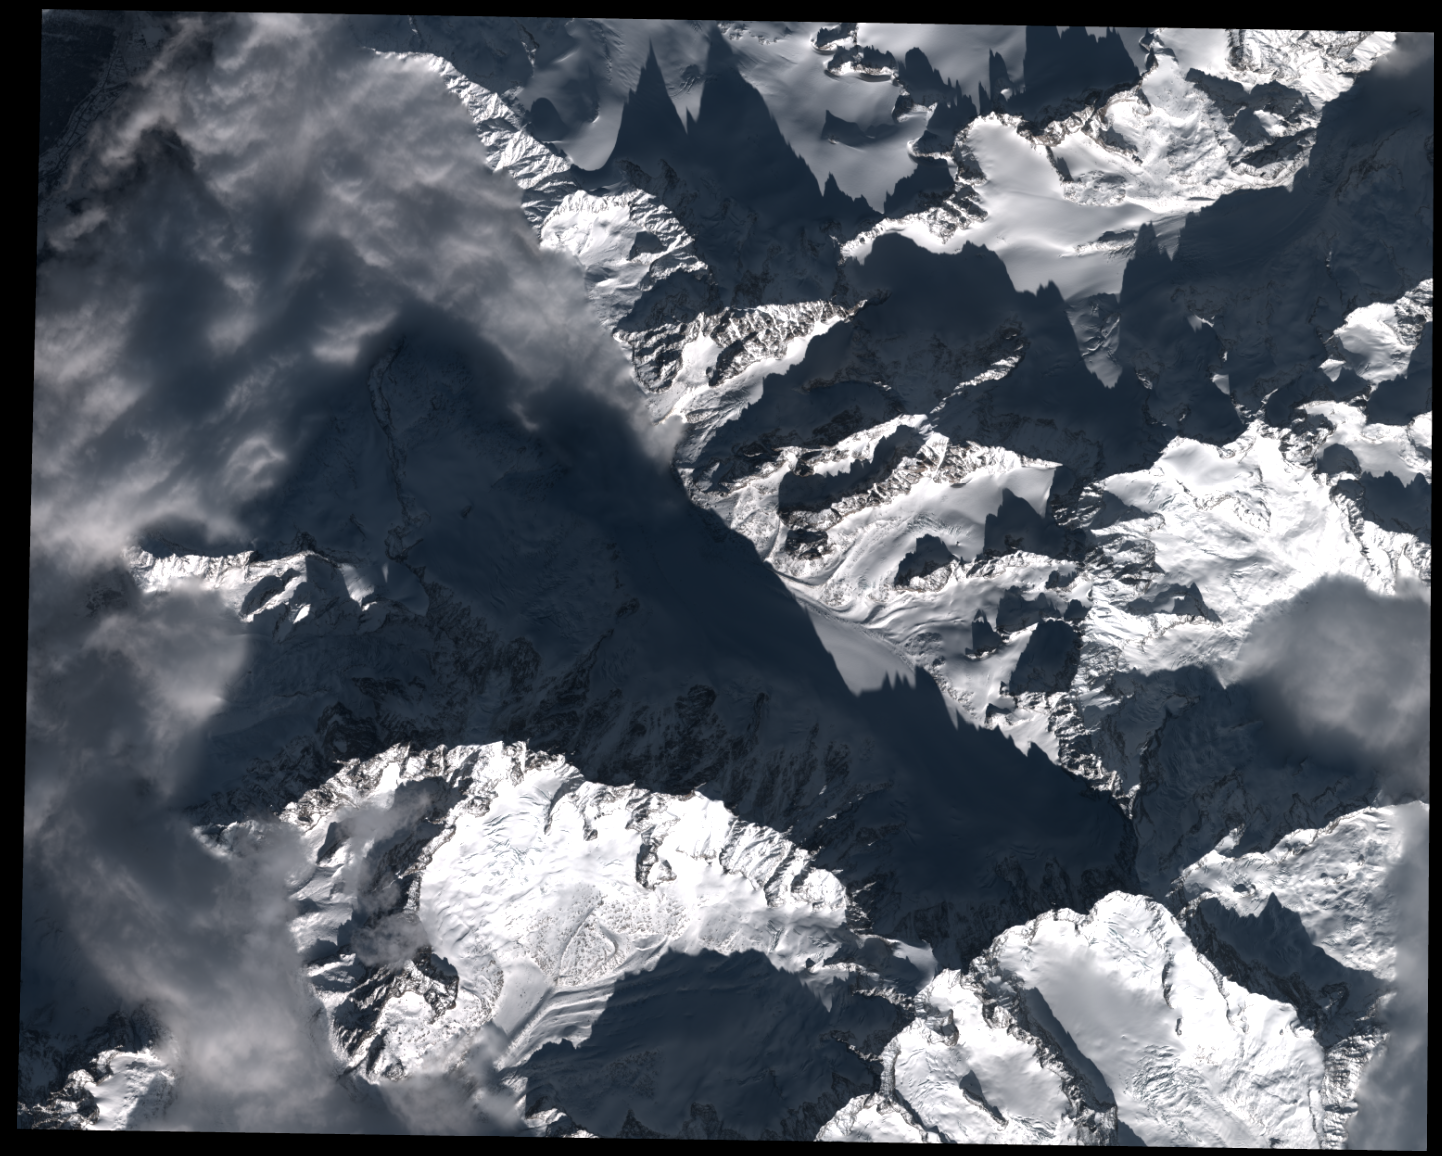
\includegraphics[keepaspectratio,width=1.005\paperwidth,height=1.1\paperheight]{images/argentiere_left.png}
\end{frame}

\vspace*{-6.5mm}
\begin{frame}[plain]
\hspace*{-11mm}
    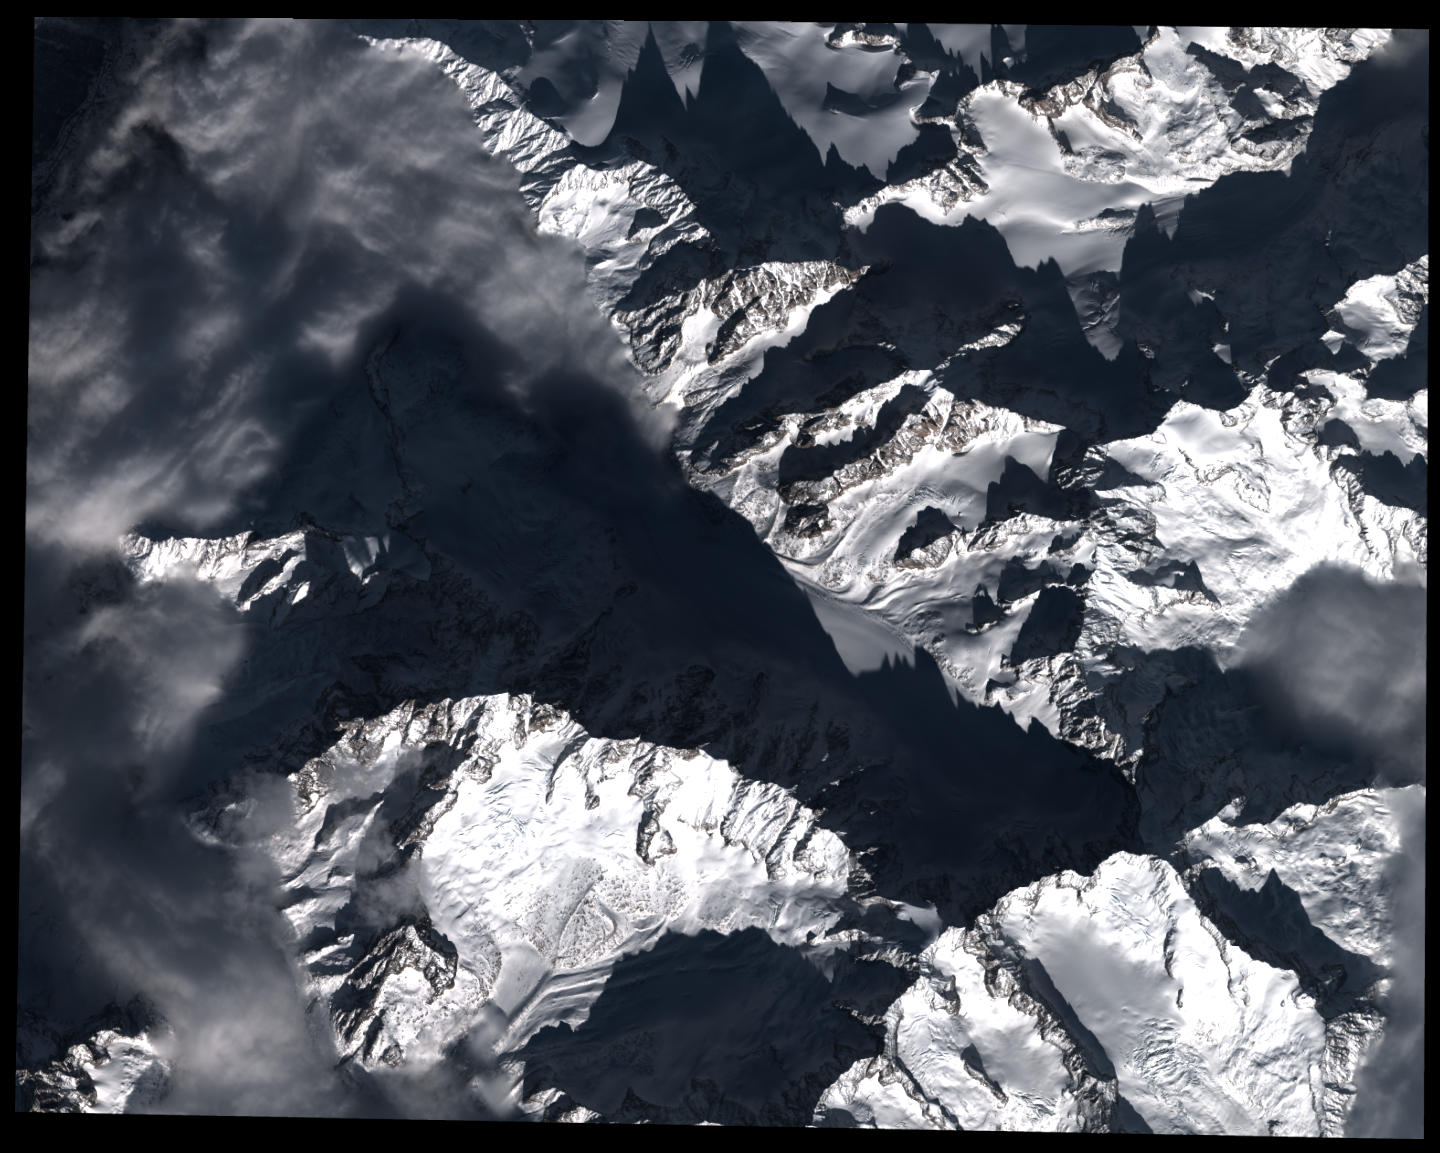
\includegraphics[keepaspectratio,width=1.005\paperwidth,height=1.1\paperheight]{images/argentiere_right.png}
\end{frame}

\vspace*{-6.5mm}
\begin{frame}[plain]
\hspace*{-11mm}
    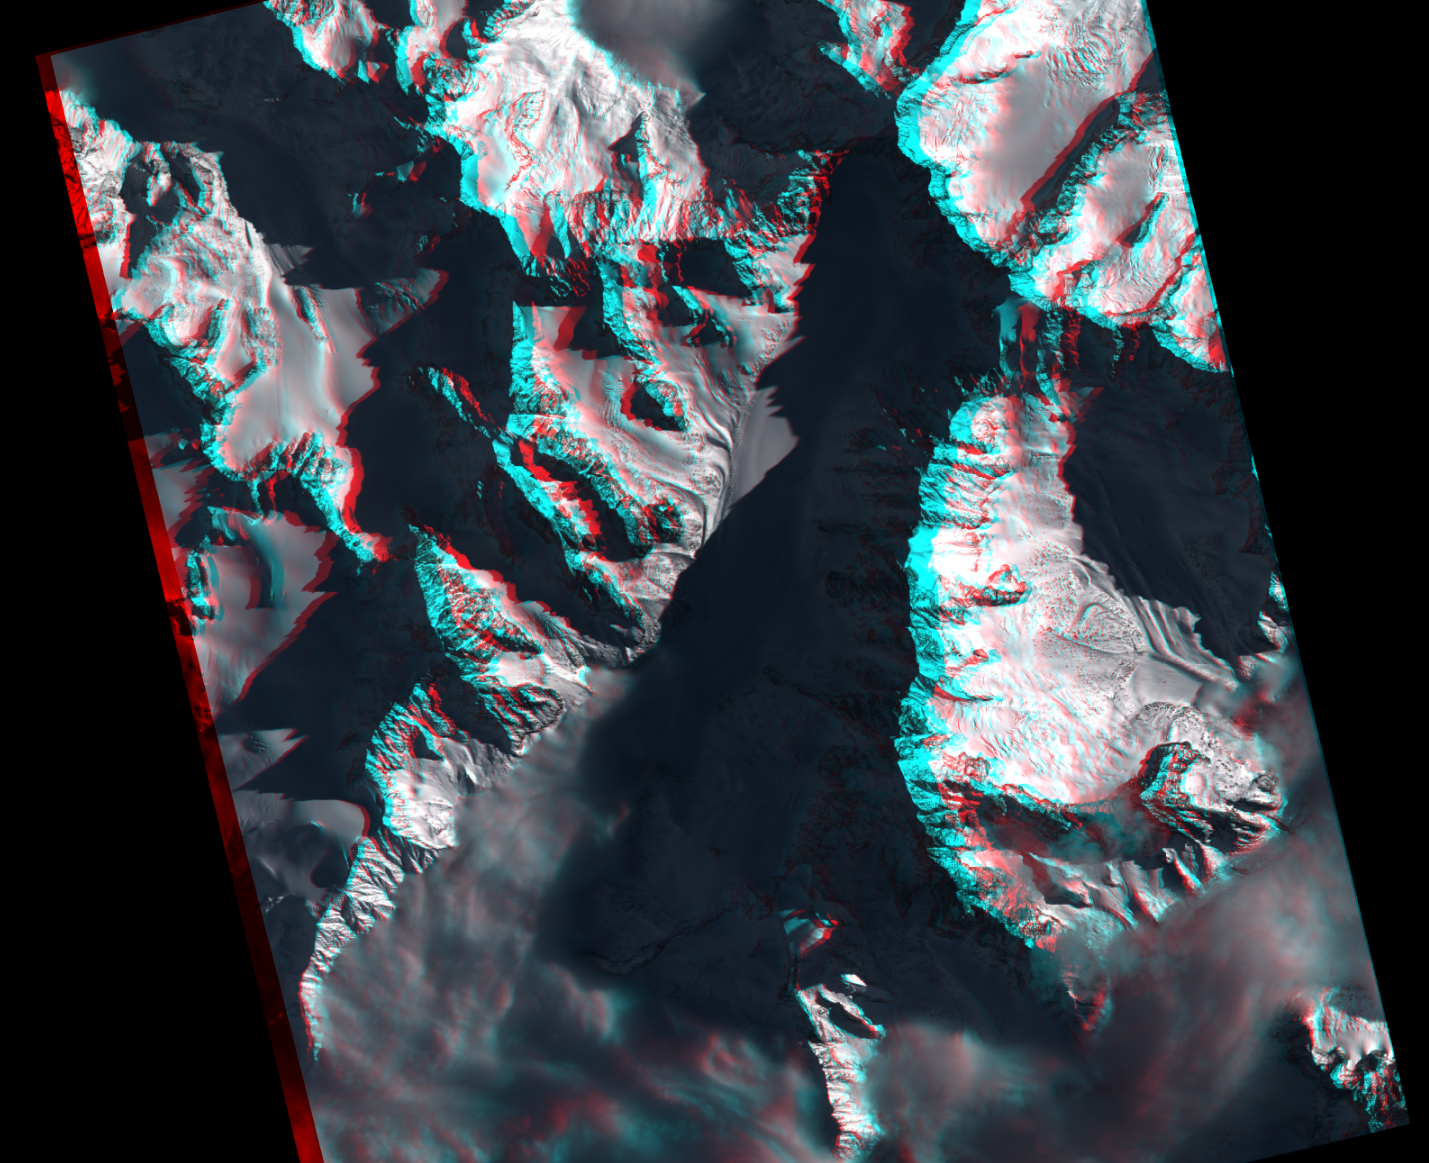
\includegraphics[keepaspectratio,width=1.005\paperwidth,height=1.1\paperheight]{images/argentiere_anaglyphe.png}
\end{frame}


\vspace*{-6.5mm}
\begin{frame}[plain]
\hspace*{-11mm}
    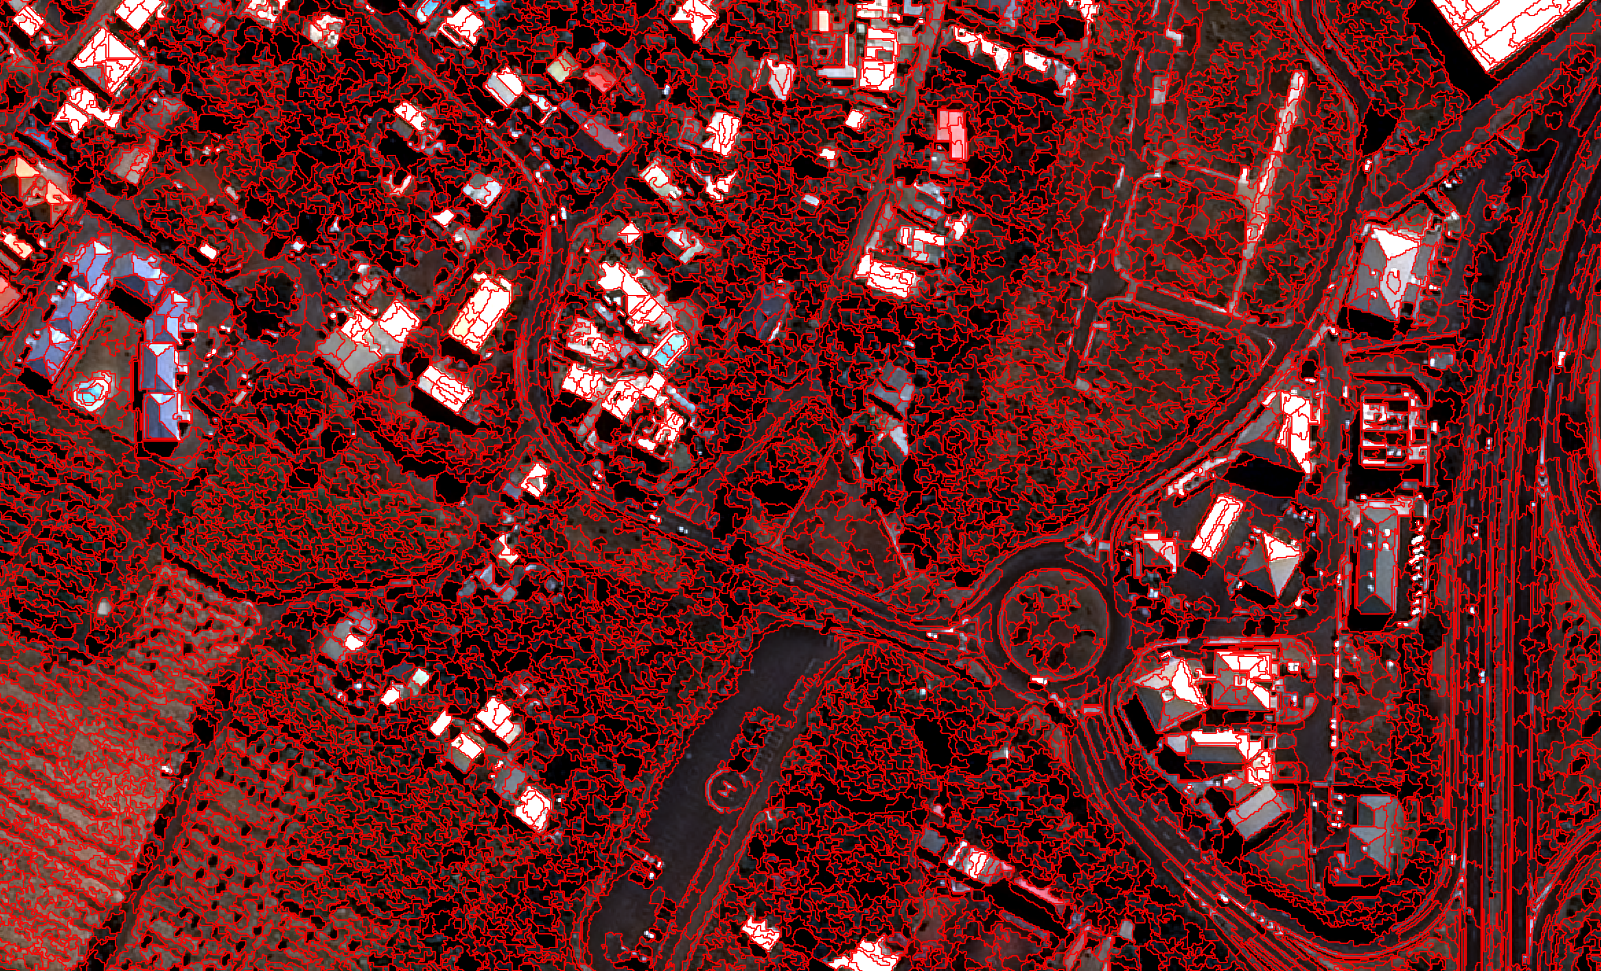
\includegraphics[keepaspectratio,height=1.1\paperheight]{images/segmentation.png}
\end{frame}

\vspace*{-6.5mm}
\begin{frame}[plain]
\hspace*{-11mm}
    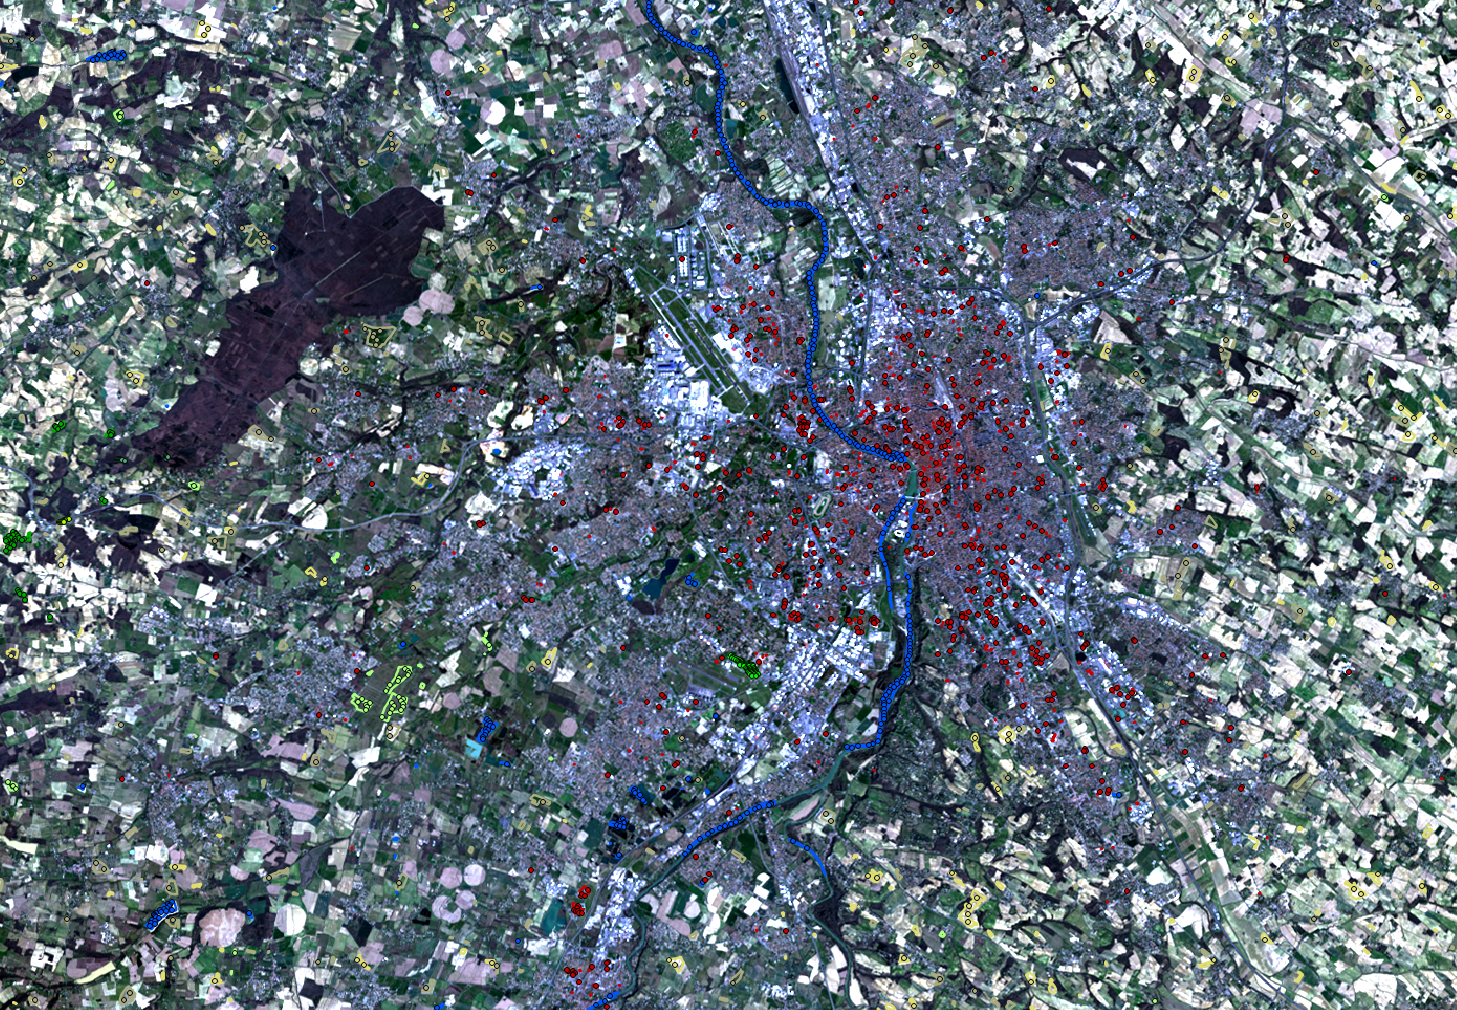
\includegraphics[keepaspectratio,height=1.1\paperheight]{../../Courses/org/WorkshopGuide/Images/samples_selection.png}
\end{frame}


\vspace*{-6.5mm}
\begin{frame}[plain]
\hspace*{-11mm}
    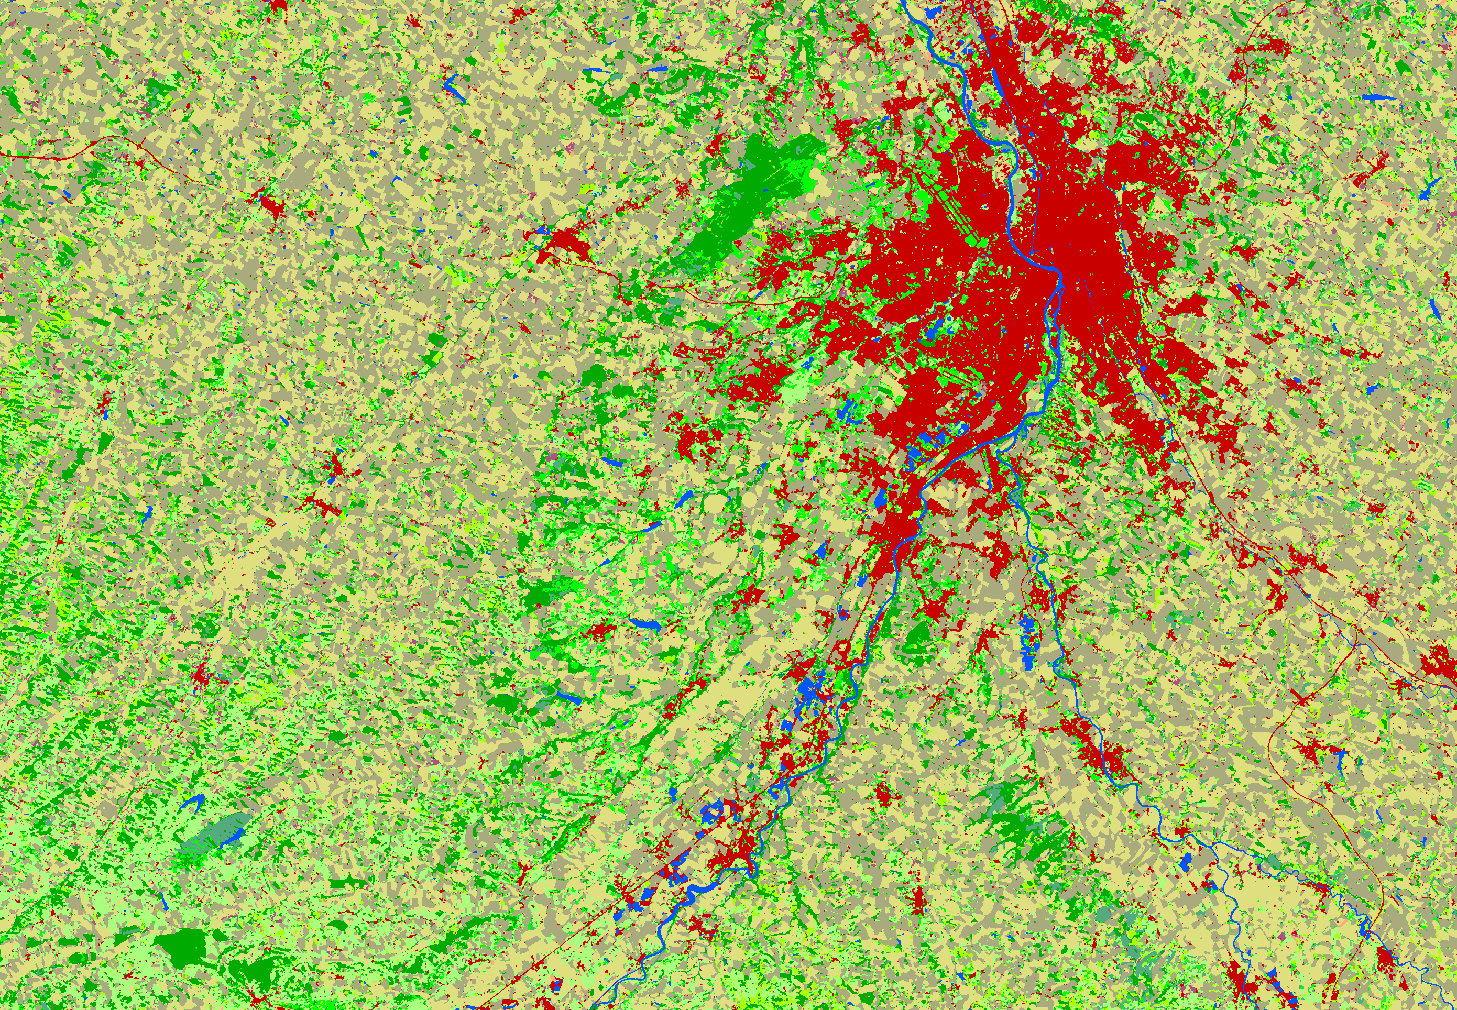
\includegraphics[keepaspectratio,height=1.1\paperheight]{../../Courses/org/WorkshopGuide/Images/final_classification.png}
\end{frame}

\vspace*{-6.5mm}
\begin{frame}[plain]
\hspace*{-11mm}
    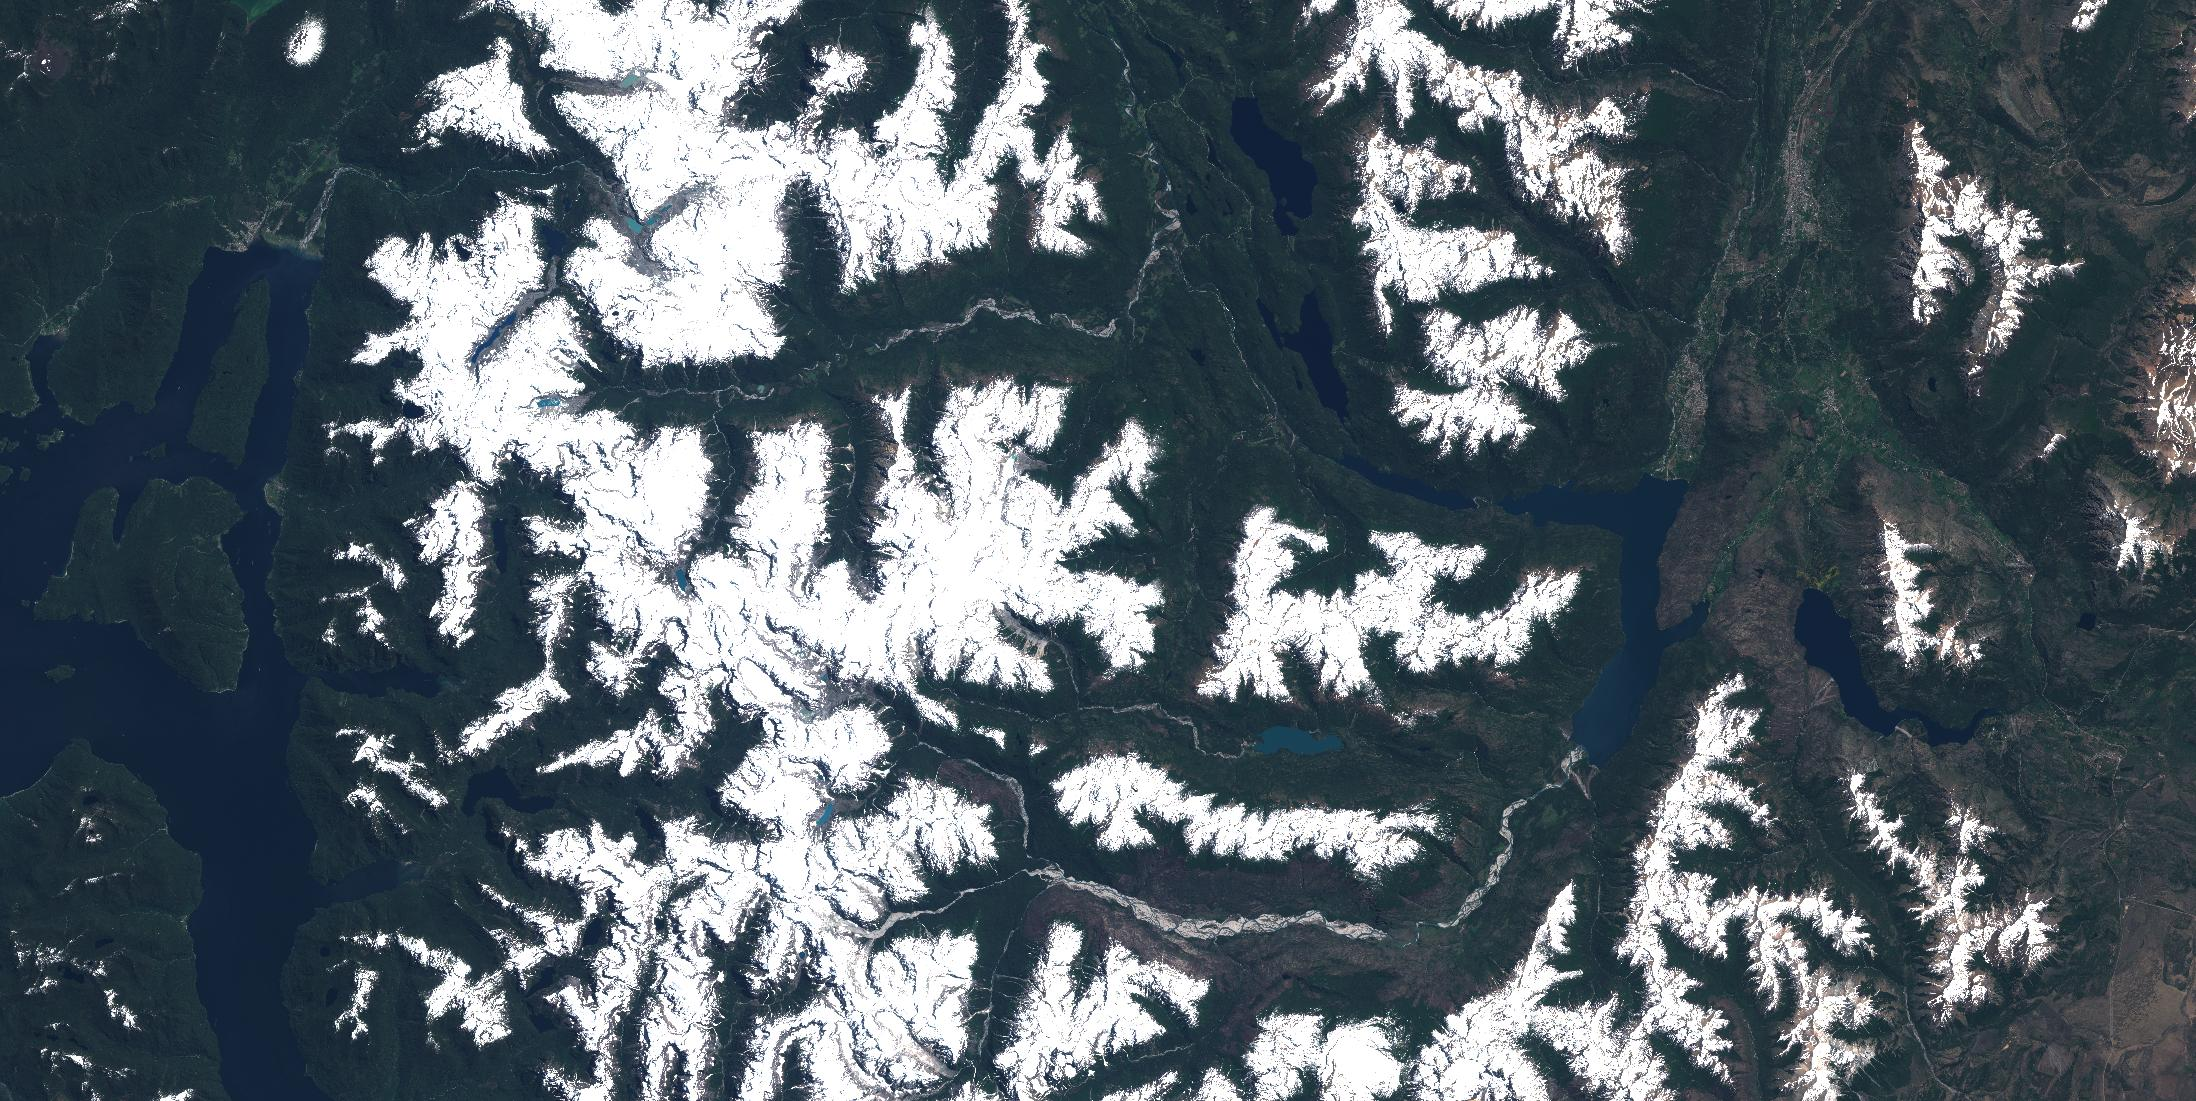
\includegraphics[keepaspectratio,height=1.1\paperheight]{images/imag4tci.jpg}
\end{frame}

\vspace*{-6.5mm}
\begin{frame}[plain]
\hspace*{-11mm}
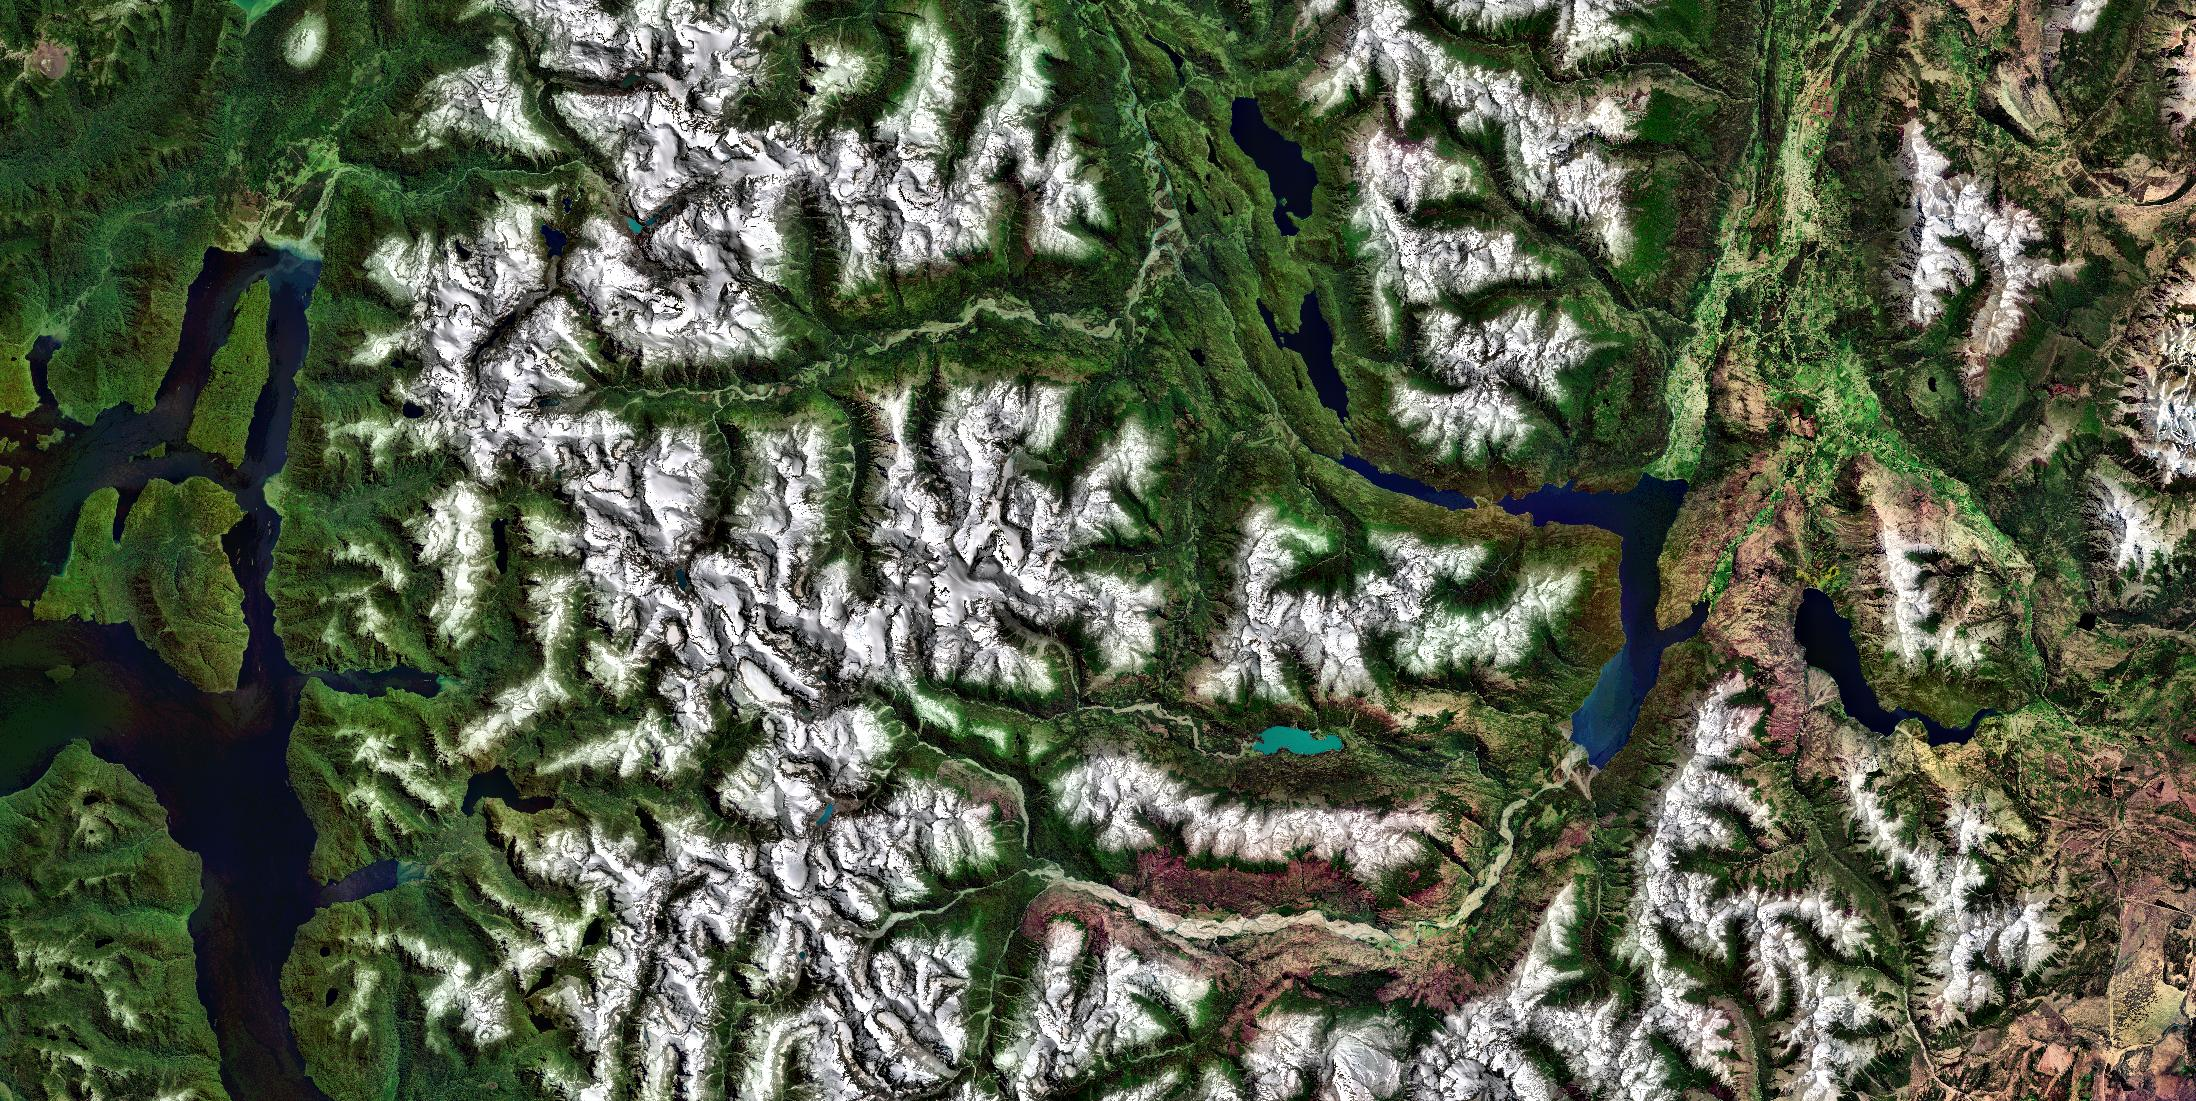
\includegraphics[keepaspectratio,height=1.1\paperheight]{images/image4_glob_each_lim20_8b_sub.jpg}
\end{frame}


\mode<all>
\section{Key characteristics}

\begin{frame}
\frametitle{Build on top of other open source image processing software}
\begin{block}{Motivations}
\begin{itemize}
\item Interfaces seamlessly with other image processing and remote sensing open-source software
\item Increase the number of functions
\item Combine tools to create hybrid data pipeline
\end{itemize}
\end{block}

\begin{block}{OTB backbone}
\begin{itemize}
\item \href{www.itk.org}{ITK}: data processing pipeline
\item \href{www.gdal.org}{GDAL}: read and write raster and vector data
\item \href{www.ossim.org}{OSSIM}: sensor modelling and metadata support
\item \href{www.opencv.org}{OpenCV} and \href{www.libsvm.org}{LibSVM}: machine learning algorithms
\item \href{www.muparser.org}{MuParser} and \href{www.muparserx.org}{MuParserX}:
  powerful parsing of mathematical expression (band math)
\end{itemize}
\end{block}

\end{frame}

\begin{frame}
\frametitle{Compatible (and available) on multiple platforms}
\begin{columns}
\column{0.5\textwidth}
\begin{block}{Goal}
\begin{itemize}
\item Compile with recent versions of:
\begin{itemize}
\item GCC
\item Clang
\item MinGW
\item Visual Studio\ldots
\end{itemize}
\item Binary packages available:
\begin{itemize}
\item UbuntuGIS repository (GIS and IP software for Ubuntu)
\item Experimental Debian packages
\item Available in  OSGeo4W (OSGeo tools on Windows)
\item Binary installers, Port and Brew formula for Mac OS X\ldots
\end{itemize}
\end{itemize}
\end{block}
\column{0.5\textwidth}
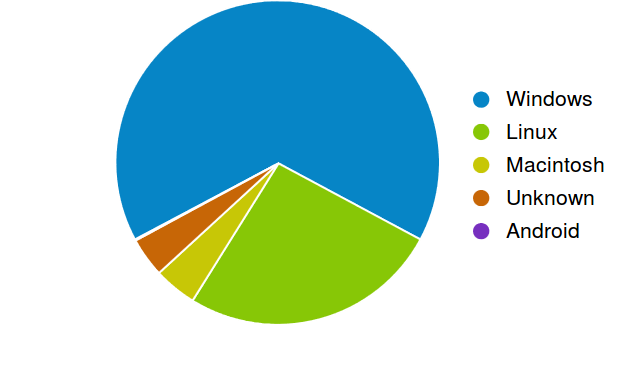
\includegraphics[width=\textwidth]{images/OTB4_download_sourceforge_os_crop.png}
\begin{center}
\tiny{Number of OTB downloads on Sourceforge per Operating System}
\end{center}
\end{columns}
\end{frame}

\begin{frame}
\frametitle{Flexibility, scalability: \textit{Pipeline}, \textit{Streaming} and \textit{multithreading}}

\begin{block}{\textit{Pipeline} data model}
\begin{center}
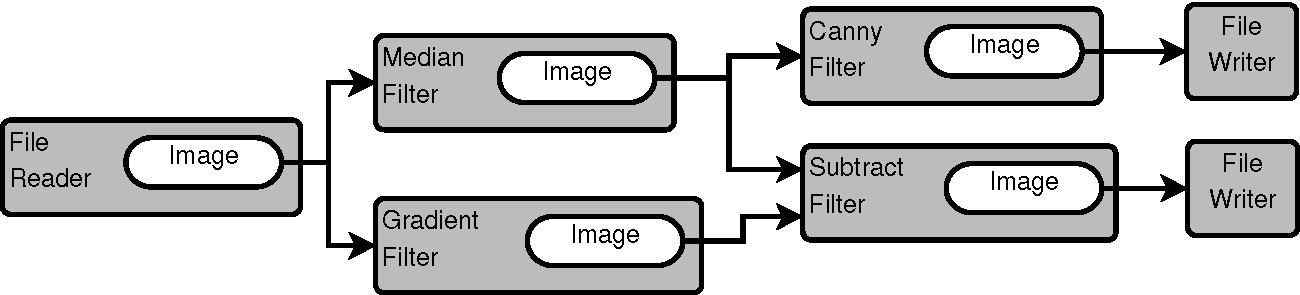
\includegraphics[width=0.7\textwidth]{images/ProcessObjectDataObject.png}
\end{center}
\end{block}
\vspace{-0.5cm}
\begin{block}{\textit{Streaming}}
\begin{center}
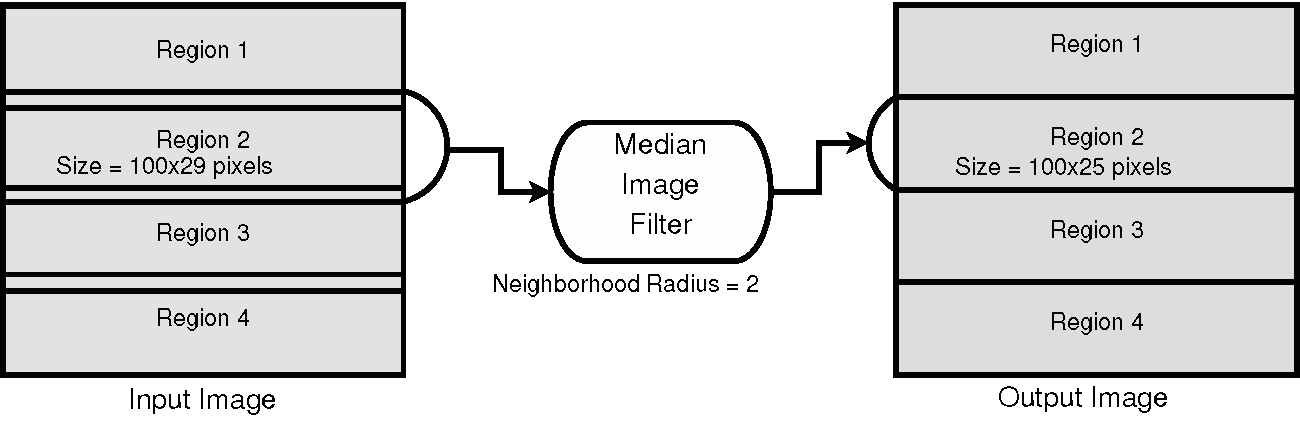
\includegraphics[width=0.7\textwidth]{images/StreamingImageDiagram.png}
\end{center}
\end{block}
\vspace{-0.5cm}
\begin{center}
\tiny{source: \url{http://www.aosabook.org/en/itk.html}}
\end{center}
\end{frame}

\begin{frame}
\frametitle{Behind the scene}
\begin{center}
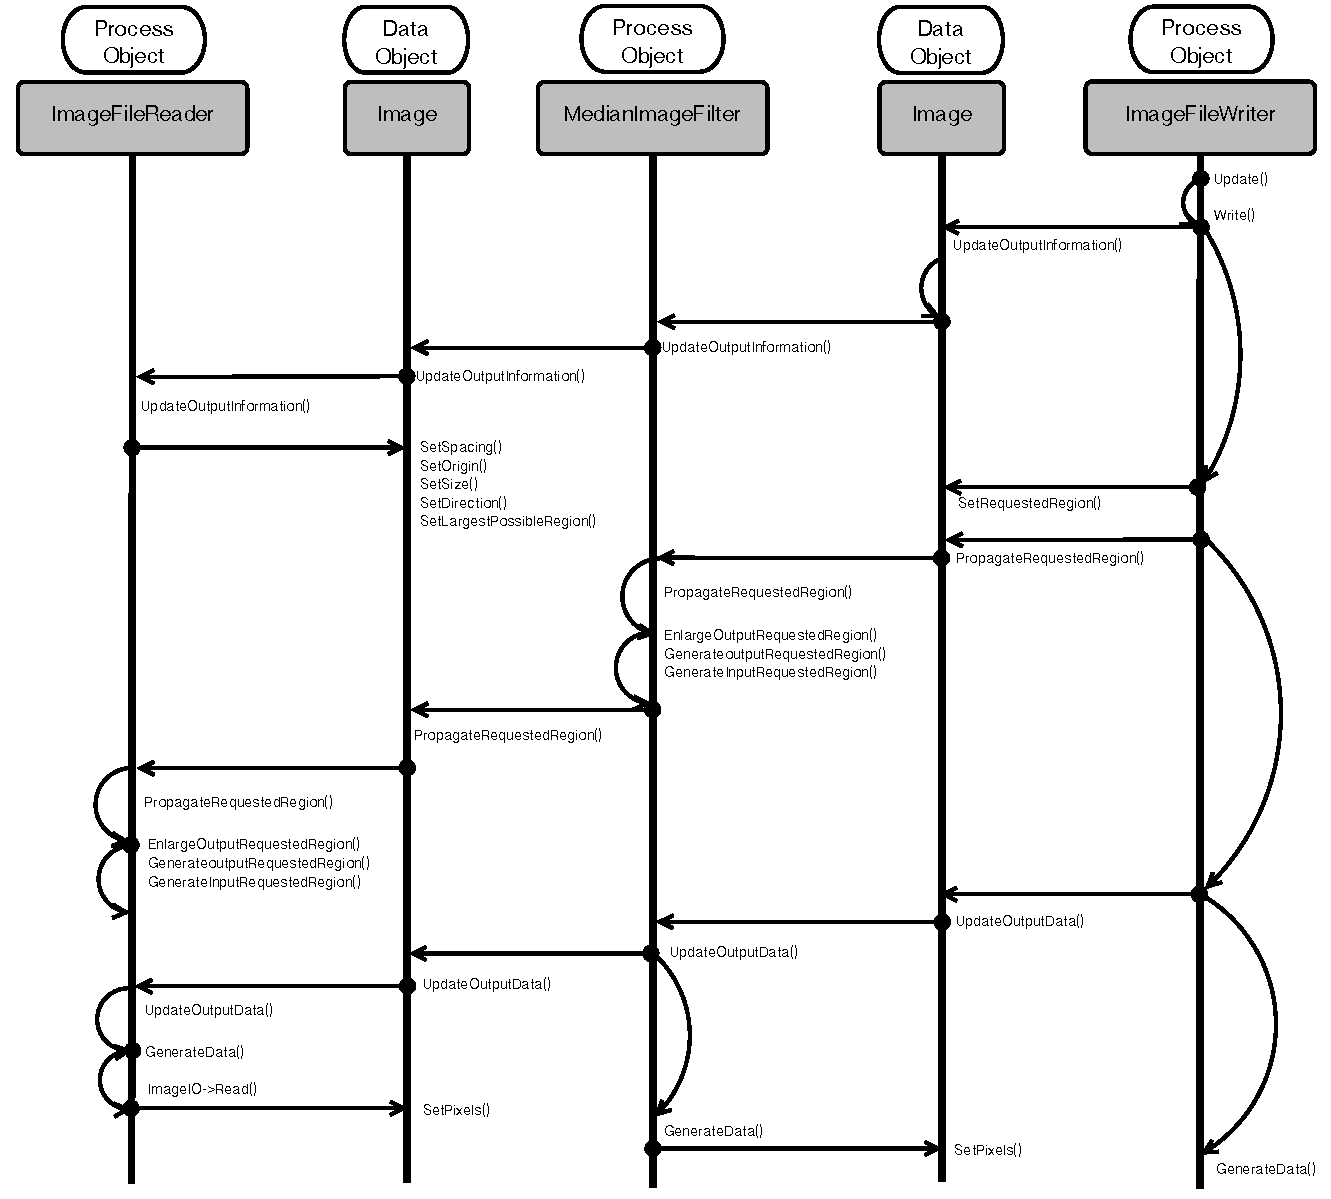
\includegraphics[width=0.7\textwidth]{images/ProcessObjectDataObjectInteractionUML.png}\\
\tiny{source: \url{http://www.aosabook.org/en/itk.html}}
\end{center}
\end{frame}

\begin{frame}
\frametitle{State of the art}
\begin{itemize}
\item Try to keep track of up-to-date information about the latest developments, exchanging ideas, identifying future trends, and making networking
\item Reference implementation of algorithms based on publications
\item e.g.: morphological profile, MeanShift segmentation, Haralick textures, SURF keypoints\ldots
\item Reference implementation contributes by authors with their
  publications. e.g.: Large Scale MeanShift, object detection \ldots
\end{itemize}
\end{frame}

\begin{frame}
\frametitle{How is OTB developed?}
\vspace{-0.5cm}
\begin{itemize}
\item Distributed version control: Git (migration from Mercurial in July 2015)
\item C++ and CMake (CTest, CDash)
\item Test driven development (TDD)
\item Agile (scrum)
\item Continuous integration and packaging
\end{itemize}
Every day, almost 3000 tests are compiled, launched on 16 different
configurations.
\begin{center}
\href{http://dash.orfeo-toolbox.org/index.php?project=OTB}{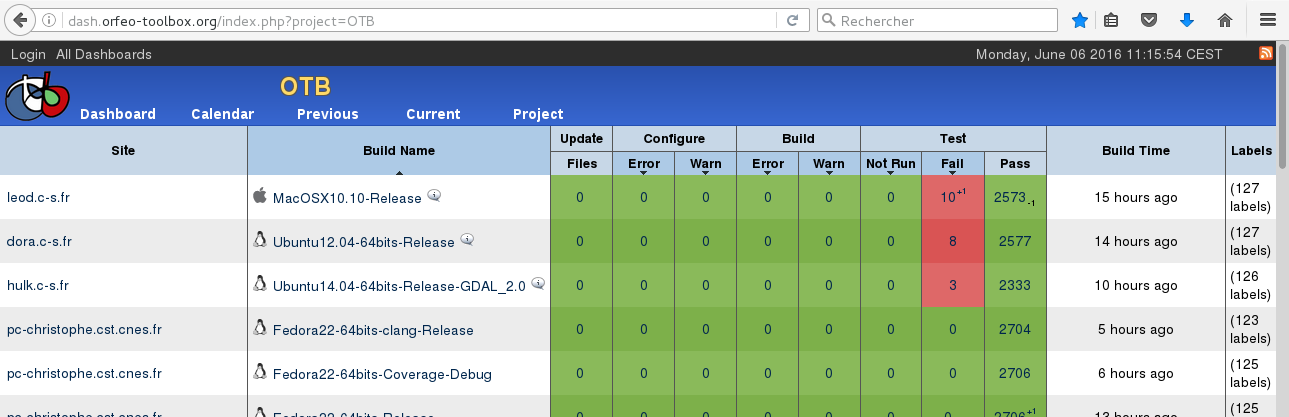
\includegraphics[width=\textwidth]{images/dashboard.png}}
\end{center}
\end{frame}


\mode<all>
\section{How to use OTB?}

\begin{frame}
\frametitle{Where to start ?}
\begin{columns}
\column{0.4\textwidth}
\begin{itemize}
\item \href{https://www.orfeo-toolbox.org}{orfeo-toolbox.org}
\item OTB CookBook :  \href{https://www.orfeo-toolbox.org/CookBook/Recipes.html}{list of recipes}
\item GitLab : \href{https://gitlab.orfeo-toolbox.org}{developer's corner}
\item Many more resources : user forum, software guide, APIs documentation, tutorials, training resources, etc.
\end{itemize}
\column{0.6\textwidth}
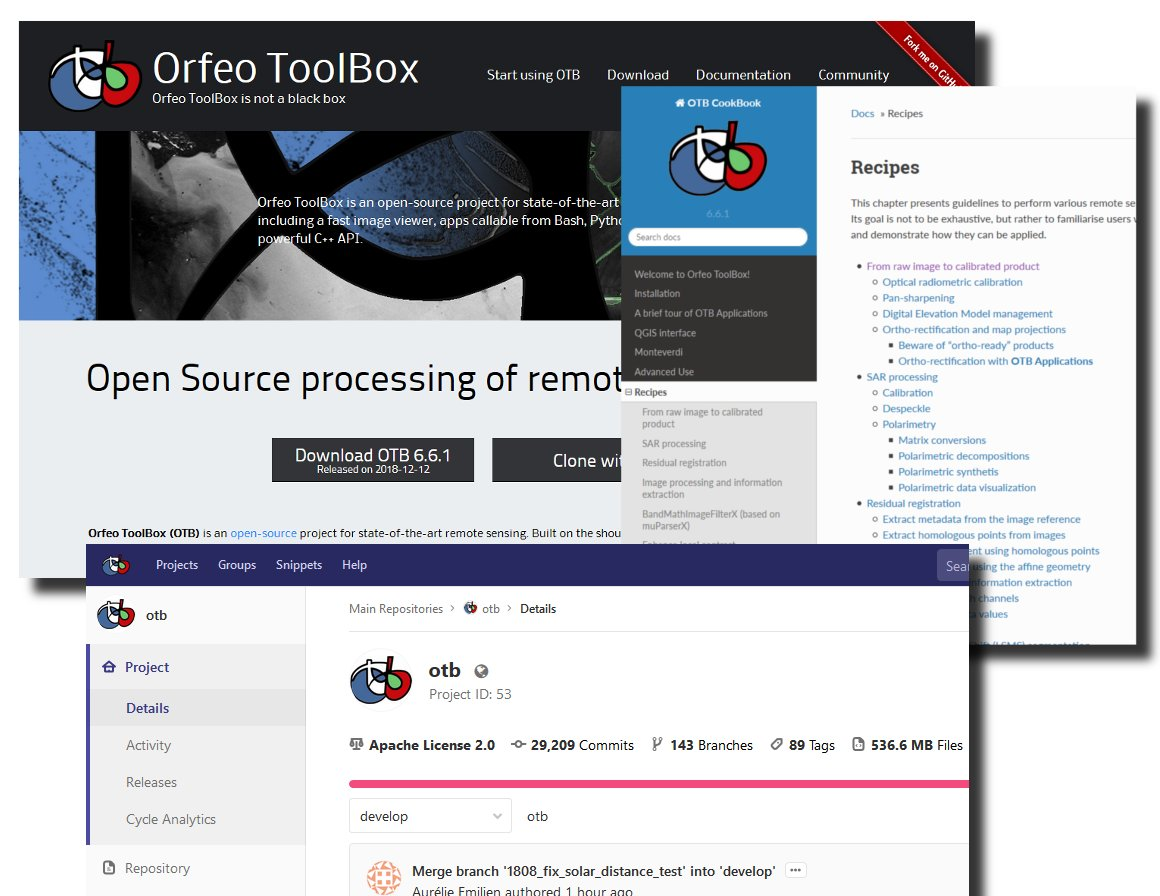
\includegraphics[width=\textwidth]{images/OTB-useful_websites.jpg}
\end{columns}
\end{frame}

\begin{frame}
\frametitle{The applications: write it once, use everywhere}
\begin{columns}
\column{0.5\textwidth}
\begin{itemize}
\item 87 applications are shipped with OTB
\item 1 application $=$ 1 dynamic library (plugin)
\item Applications are auto-descriptive and auto-documented
\item Applications can be extended outside of OTB
\item Several plugins players:
\begin{itemize}
  \item Command-line
  \item Qt auto-generated
  \item Python
\end{itemize}
\item Applications are meant for integration in external systems
\end{itemize}
\column{0.5\textwidth}
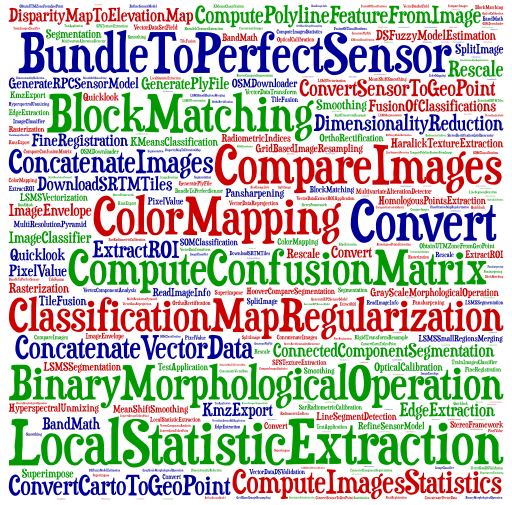
\includegraphics[width=\textwidth]{../OTB-General/images/cloud_applications.png}
\end{columns}
\end{frame}


\begin{frame}
\frametitle{How to use OTB?}
\vspace{-0.5cm}
\begin{center}
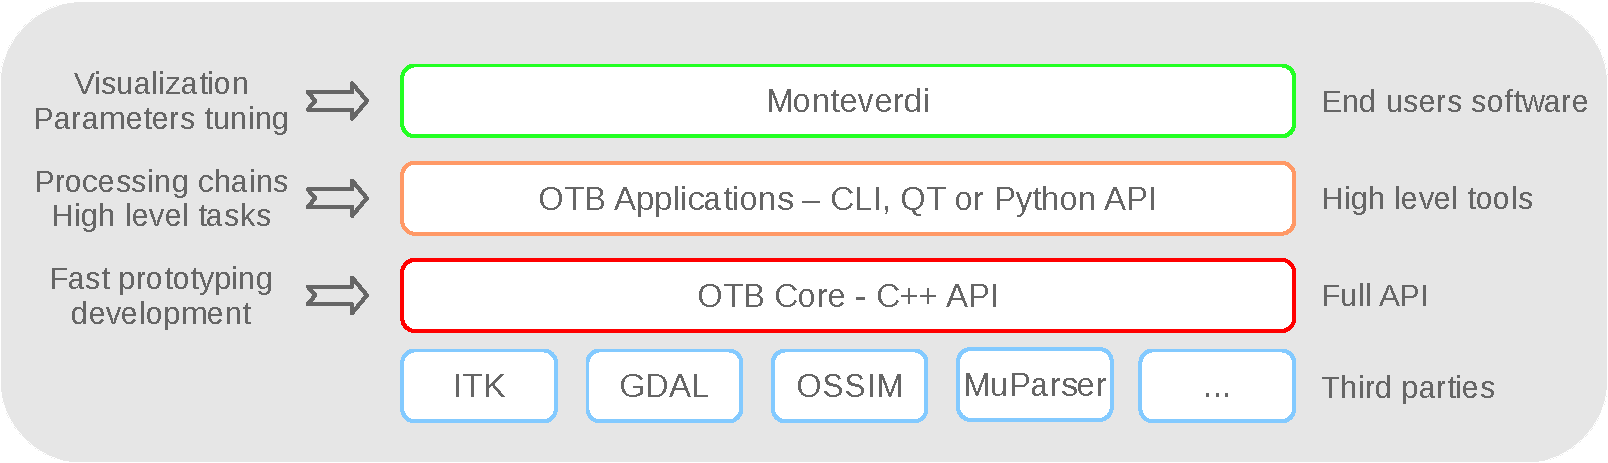
\includegraphics[width=\textwidth]{../OTB-General/images/sandwich.pdf}
\end{center}
\vspace{-0.5cm}
\begin{block}{Use Monteverdi (or QGIS !)}
Visualization, data management, \textcolor{red}{Access to all applications}
\end{block}
\begin{block}{Use the applications}
 High level functions (e.g. segmentation), callable from CLI, Qt, Python, can be extended
\end{block}
\begin{block}{Write your own code}
 Flexible, access to full API, requires C++ knowledge
\end{block}

\end{frame}

\begin{frame}[fragile]
\frametitle{Show me the code!}
\begin{lstlisting}[language=c++,breaklines=true,breakatwhitespace=true,frame = tb,framerule = 0.25pt,fontadjust,backgroundcolor={\color{listlightgray}},basicstyle = {\ttfamily\tiny},keywordstyle = {\ttfamily\color{red}\textbf},identifierstyle = {\ttfamily},commentstyle = {\ttfamily\color{listcomment}\textit},stringstyle = {\ttfamily},showstringspaces = false,showtabs = false,numbers = none,numbersep = 2pt, numberstyle={\ttfamily\color{listnumbers}},tabsize = 2]
#include "otbImage.h"
#include "otbImageFileReader.h"
#include "otbImageFileWriter.h"
#include "itkCannyEdgeDetectionImageFilter.h"
#include "itkRescaleIntensityImageFilter.h"

int main(int argc, char * argv[])
{
  typedef double                      PixelType;
  typedef otb::Image<PixelType>       ImageType;

  typedef unsigned char               OutputPixelType;
  typedef otb::Image<OutputPixelType> OutputImageType;

  typedef otb::ImageFileReader<ImageType> ReaderType;
  ReaderType::Pointer reader = ReaderType::New();

  reader->SetFileName(argv[1]);

  typedef itk::CannyEdgeDetectionImageFilter
  <ImageType, ImageType> FilterType;
  FilterType::Pointer filter = FilterType::New();

  filter->SetInput(reader->GetOutput());

  typedef otb::ImageFileWriter<OutputImageType> WriterType;
  WriterType::Pointer writer = WriterType::New();

  writer->SetFileName(argv[2]);

  writer->SetInput(filter->GetOutput());

  writer->Update();
}
\end{lstlisting}
\end{frame}





\begin{frame}[fragile]
\frametitle{Applications: command-line invocation}
\begin{scriptsize}
\vspace{-0.5cm}\begin{verbatim}
$ otbcli_OrthoRectification

ERROR: Waiting for at least one parameter...
This is the OrthoRectification application, version 5.2.1
This application allows to ortho-rectify optical images from supported sensors.

Complete documentation: http://www.orfeo-toolbox.org/Applications/OrthoRectification.html

Parameters:
        -progress                <boolean>        Report progress
MISSING -io.in                   <string>         Input Image  (mandatory)
MISSING -io.out                  <string> [pixel] Output Image  [pixel=uint8/uint16/int16/uint32/int32/float/double] (default value is float) (mandatory)
        -map                     <string>         Output Cartographic Map Projection [utm/lambert2/lambert93/wgs/epsg] (mandatory, default value is utm)
        -map.utm.zone            <int32>          Zone number  (mandatory, default value is 31)
        -map.utm.northhem        <boolean>        Northern Hemisphere  (optional, off by default)
        -map.epsg.code           <int32>          EPSG Code  (mandatory, default value is 4326)
        -outputs.mode            <string>         Parameters estimation modes [auto/autosize/autospacing/outputroi/orthofit] (mandatory, default value is auto)
MISSING -outputs.ulx             <float>          Upper Left X  (mandatory)
MISSING -outputs.uly             <float>          Upper Left Y  (mandatory)
MISSING -outputs.sizex           <int32>          Size X  (mandatory)
MISSING -outputs.sizey           <int32>          Size Y  (mandatory)
MISSING -outputs.spacingx        <float>          Pixel Size X  (mandatory)
MISSING -outputs.spacingy        <float>          Pixel Size Y  (mandatory)
        -outputs.lrx             <float>          Lower right X  (optional, off by default)
        -outputs.lry             <float>          Lower right Y  (optional, off by default)
        -outputs.ortho           <string>         Model ortho-image  (optional, off by default)
        -outputs.isotropic       <boolean>        Force isotropic spacing by default  (optional, on by default)
        -outputs.default         <float>          Default pixel value  (optional, on by default, default value is 0)
        -elev.dem                <string>         DEM directory  (optional, off by default)
        -elev.geoid              <string>         Geoid File  (optional, off by default)
        -elev.default            <float>          Default elevation  (mandatory, default value is 0)
        -interpolator            <string>         Interpolation [bco/nn/linear] (mandatory, default value is bco)
\end{verbatim}
\end{scriptsize}
\end{frame}


\begin{frame}[fragile]
\frametitle{Applications: Graphical interface}
\begin{center}
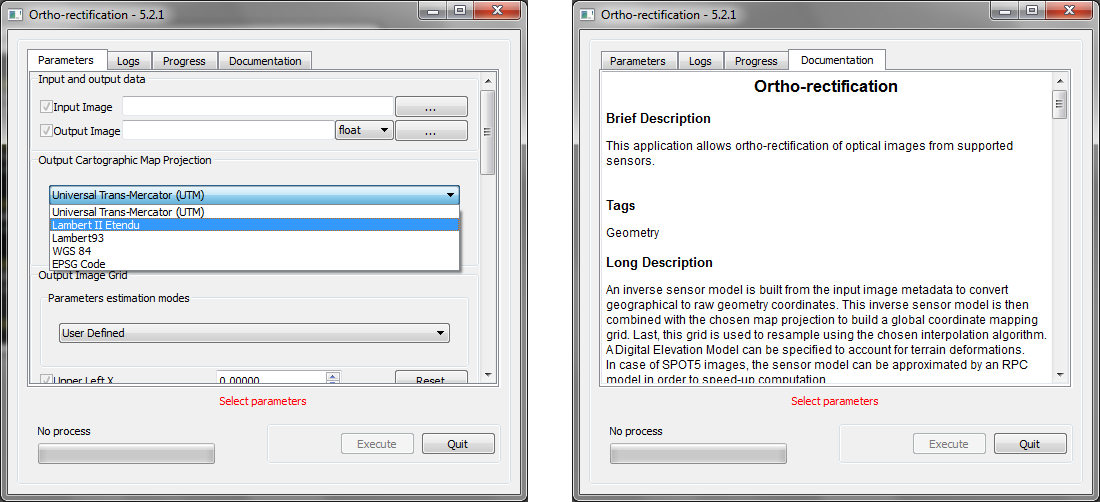
\includegraphics[width=1\textwidth]{../OTB-General/images/otbgui.png}
\end{center}
\end{frame}

\begin{frame}[fragile]
\frametitle{Applications: Python interface}
\begin{lstlisting}[language=python,breaklines=true,breakatwhitespace=true,frame = tb,framerule = 0.25pt,fontadjust,backgroundcolor={\color{listlightgray}},basicstyle = {\ttfamily\tiny},keywordstyle = {\ttfamily\color{listkeyword}\textbf},identifierstyle = {\ttfamily},commentstyle = {\ttfamily\color{listcomment}\textit},stringstyle = {\ttfamily},showstringspaces = false,showtabs = false,numbers = none,numbersep = 6pt, numberstyle={\ttfamily\color{listnumbers}},tabsize = 2]
#!/usr/bin/python

# Import the otb applications package
import otbApplication

# The following line creates an instance of the OrthoRectification application
OrthoRectification = otb.Registry.CreateApplication("OrthoRectification")

# The following lines set all the application parameters:
OrthoRectification.IO.IN = "QB_TOULOUSE_MUL_Extract_500_500.tif"
OrthoRectification.IO.OUT = "QB_Toulouse_ortho.tif"

app.MAP = 'epsg'
app.MAP.EPSG.CODE = 32768

# The following line execute the application
OrthoRectification.ExecuteAndWriteOutput()
\end{lstlisting}
\end{frame}


\begin{frame}
\frametitle{Monteverdi (acces to OTB applications)}
\begin{minipage}[t][6cm][t]{\textwidth}
\begin{center}
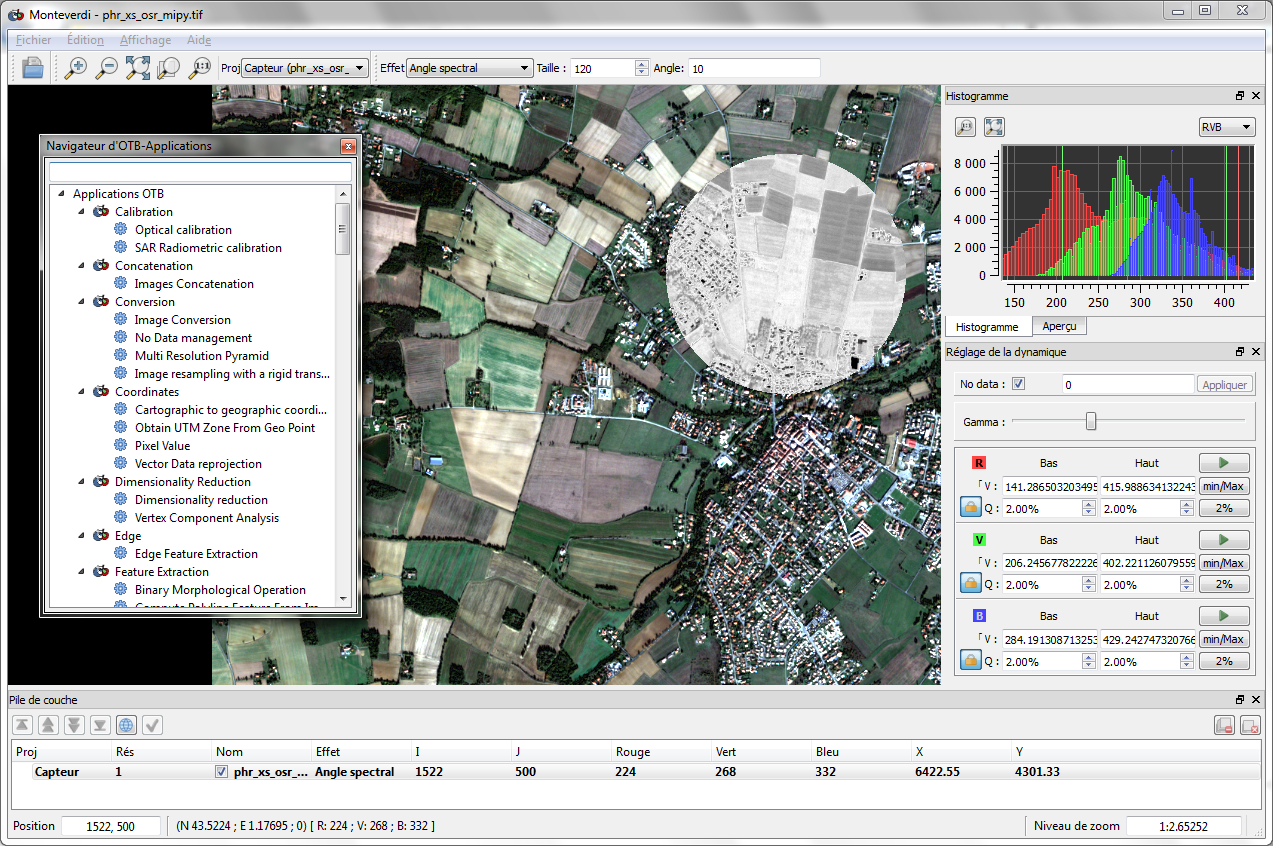
\includegraphics[width=1.0\textwidth]{../OTB-General/images/monteverdi.png}
\end{center}
\end{minipage}
\end{frame}

%\vspace*{-3.0mm}
\begin{frame}
  \frametitle{QGIS}
\begin{minipage}[t][6cm][t]{\textwidth}
\begin{center}
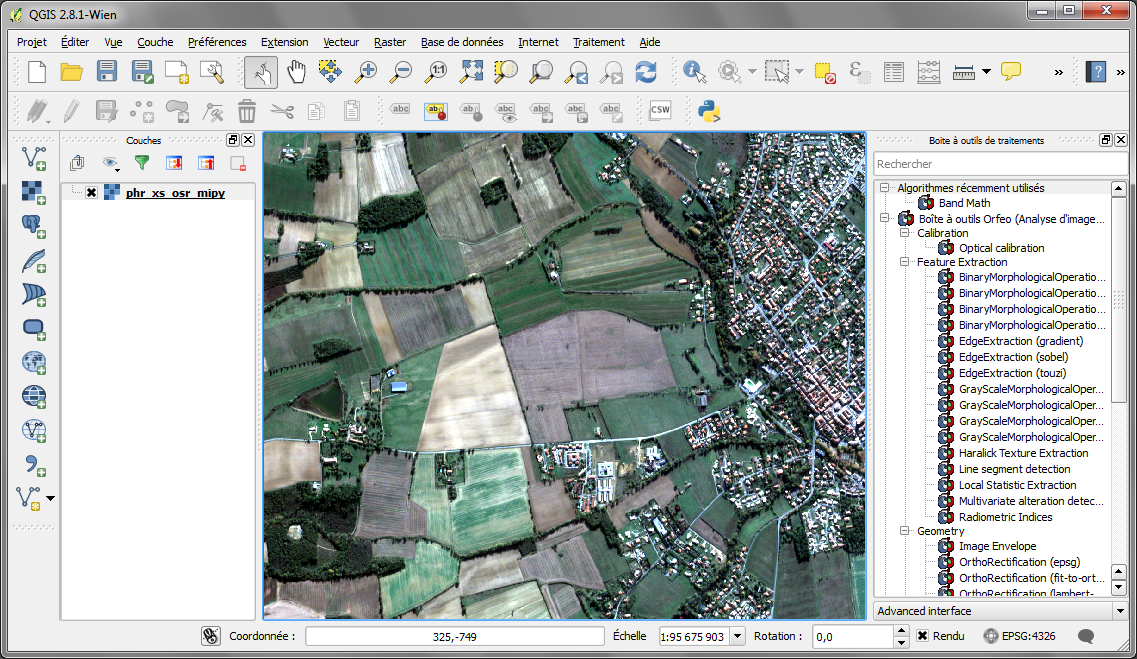
\includegraphics[width=1\textwidth]{../OTB-General/images/otb_in_qgis.png}
\end{center}
\end{minipage}
\end{frame}



\mode<all>
\section{What's new in OTB?}

\mode<all>
\begin{frame}
\frametitle{5.0 (May 2015)}
\begin{block}{Make OTB more modular}
\begin{itemize}
  \item Better code layout, coherent modules (124 modules and 16 groups) with
    source, test and applications.
\item Dependency management
\item External contributions: \url{https://www.orfeo-toolbox.org/external-projects/}
\end{itemize}
\end{block}

\begin{block}{SuperBuild}
\begin{itemize}
\item No more third party software in OTB!
\item The Superbuild downloads, configures, builds and installs dependencies
\item Offline mode for compiling OTB without network access (e.g. airplane)
\end{itemize}
\end{block}
\end{frame}

\begin{frame}
\frametitle{Open governance: Project Steering Committee}
\begin{block}{PSC beginning}
  \begin{itemize}
  \item Until 2015: OTB is open-source software
  \item In march 2015: OTB become free software, with CNES as the first PSC
  \end{itemize}
\end{block}
\begin{block}{A club of developers, not managers}
  \begin{itemize}
  \item High level project steering, roadmaps, communication and planning
  \item Vote RFCs: all members' votes have the same value ($\pm 1$, $\pm 0$)
  \item Seats do not expire. Exits are by resignation or vote of expulsion
  \item The PSC is not a legal entity and has no funding
  \end{itemize}
\end{block}
\begin{block}{Numbers}
  \begin{itemize}
  \item 5 members from 4 different organizations
  \item 2 releases under a PSC (5.2, 5.4)
  \item 3 online meetings (with public logs)
  \end{itemize}
\end{block}
\end{frame}


\mode<all>
\begin{frame}
\frametitle{5.2 (December 2015)}
\begin{block}{OTB}
\begin{itemize}
\item New SAR processing applications (polarimetry, radiometry, speckle)
\item Support for Sentinel-1 products (radiometric calibration)
\item Better Python bindings
\item Better GDAL 2.0 compatibility and support Sentinel-2 images
\item Official package in DebianGIS (special thanks to Rashad and Debian maintainer)
\item \ldots
\end{itemize}
\end{block}

\begin{block}{Monteverdi 3.0}
\begin{itemize}
\item Display an image mosaic or multi-temporal dataset
\item Efficient visualization tools (local contrast, gradient \ldots)
\item Access to OTB applications
\end{itemize}
\end{block}
\end{frame}


\mode<all>
\begin{frame}
\frametitle{5.4 (May 2016)}
\begin{block}{OTB}
\begin{itemize}
\item Switched to a fixed release schedule
\item Merged Ice (visualization lib) into OTB
\item External build of external modules
\item New SAR decomposition methods: Barnes, Huynen, Pauli
\end{itemize}
\end{block}

\begin{block}{Monteverdi 3.2}
\begin{itemize}
\item Screen-shot feature
\item Generate GDAL overviews
\item Support for GDAL sub-datasets
\item Added to the SuperBuild
\end{itemize}
\end{block}
\end{frame}


\mode<all>
\begin{frame}
\frametitle{5.6 (August 2016)}
\begin{block}{OTB}
\begin{itemize}
\item MPI pipeline execution
\item Samples extractor and selection for supervised classification
\item Improve classification on vector
\item Support for Sentinel-1 products (geometric calibration)
\end{itemize}
\end{block}

\begin{block}{Monteverdi 3.4}
\begin{itemize}
\item Improve OTB-applications display \& search bar
\end{itemize}
\end{block}
\end{frame}

\begin{frame}[fragile]
\frametitle{Parallel OTB pipeline with MPI}
  \begin{center}
  \vspace{-0.5cm}
  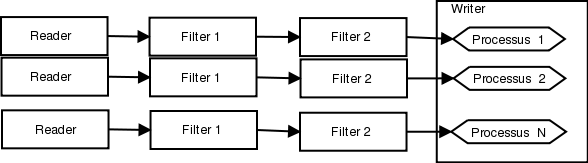
\includegraphics[width=0.6\textwidth]{images/mpi.png}
  \begin{scriptsize}
\begin{verbatim}
    $ mpirun -np $nb_procs --hostfile $PBS_NODEFILE  \
    otbcli_BundleToPerfectSensor \
    -inp $ROOT/IMG_PHR1A_P_001/IMG_PHR1A_P_201605260427149_ORT_1792732101-001_R1C1.JP2 \
    -inxs $ROOT/IMG_PHR1A_MS_002/IMG_PHR1A_MS_201605260427149_ORT_1792732101-002_R1C1.JP2 \
    -out $ROOT/pxs.tif uint16 -ram 1024

    ------------ JOB INFO 1043196.tu-adm01 -------------
    
    JOBID           : 1043196.tu-adm01
    USER            : michelj
    GROUP           : ctsiap
    JOB NAME        : OTB_mpi
    SESSION         : 631249
    RES REQSTED     : mem=1575000mb,ncpus=560,place=free,walltime=04:00:00
    RES USED        : cpupercent=1553,cput=00:56:12,mem=4784872kb,ncpus=560,vmem=18558416kb,
    walltime=00:04:35
    BILLING         : 42:46:40 (ncpus x walltime)
    QUEUE           : t72h
    ACCOUNT         : null
    JOB EXIT CODE   : 0
    
    ------------ END JOB INFO 1043196.tu-adm01 ---------
\end{verbatim}
\end{scriptsize}
\end{center}
\end{frame}


\mode<all>
\begin{frame}
\frametitle{5.8 (October 2016)}
\begin{block}{OTB}
\begin{itemize}
\item Access to Shark random forests (better performances, parallel learning)
\item Better performances in BandMathX
\item Spot7 support (radiometric and geometric calibration)
\item Applications in-memory connection
\item Full new classification framework available
\item And lots of other small improvements ...
\end{itemize}
\end{block}

\begin{block}{Monteverdi}
\begin{itemize}
\item Now part of OTB source code
\item Zoom with mouse wheel without CTRL
\end{itemize}
\end{block}
\end{frame}


\mode<all>
\begin{frame}
  \frametitle{5.10 (February 2017)}
  \begin{block}{OTB}
    \begin{itemize}
      \item Composite applications framework 
      \item TrainImagesClassifier and BundleToPerfectSensor refactoring (composite)
      \item Print corresponding command-line in apps QT GUI
      \item Enhancement of field selector QT component
      \item FFT/DWT application
      \item Texture app now allows for subsampled results (faster)
    \end{itemize}
  \end{block}
  
  \begin{block}{Monteverdi}
    \begin{itemize}
      \item Single band color mapping
      \end{itemize}
  \end{block}
      
\end{frame}


\mode<all>
\begin{frame}
  \frametitle{6.0 (May 2017)}
  \begin{block}{OTB}
    \begin{itemize}
      \item Licence change to  Apache v2.0
      \item OpenCV 3.0 support
      \item Sentinel1 IW SLC deburst application
      \item Band selection through extended filenames
      \item Unsupervised classification in framework
      \item Morphological profiles app
      \item Vector files classification app
      \item Deprecated code cleanup (major release)
    \end{itemize}
    \end{block}
\end{frame}


\mode<all>
\begin{frame}
  \frametitle{6.2 (October 2017)}
  \begin{block}{OTB}
    \begin{itemize}
      \item Better help, doc and logs
      \item \textit{All in one} LSMS segmentation
      \item Improvements and refactoring of several applications: Convert, DownloadSRTMTiles, PixelValue, ExtractROI
      \item Binary packages include files needed to develop with OTB
      \item OTB has graduated in July from incubation and is now a full fledged OSGeo project!
    \end{itemize}
    \end{block}
\end{frame}


\mode<all>
\begin{frame}
  \frametitle{6.4 (January 2018)}

  \begin{itemize}
  \item Enhancement of multiple files selection widget
  \item Application and filter for local contrast enhancement (CLAHE)
  \item Improvement of generic SAR sensor model
  \item Python 3 support
  \item After this release: moving to gitlab!
  \end{itemize}  
\end{frame}

\begin{frame}
  \frametitle{Gitlab: easier, more integrated}
  \begin{columns}
    \column{0.4\textwidth}
    \begin{itemize}
    \item Request for comments, bugs, feature requests $\Rightarrow$ gitlab issues
    \item All code modifications goes through Merge Requests
    \item Easier code review, links between issues and Merge Requests
    \item Code contribution more straightforward
    \item Provides hosting for Remote Modules
    \end{itemize}
    \column{0.6\textwidth}
    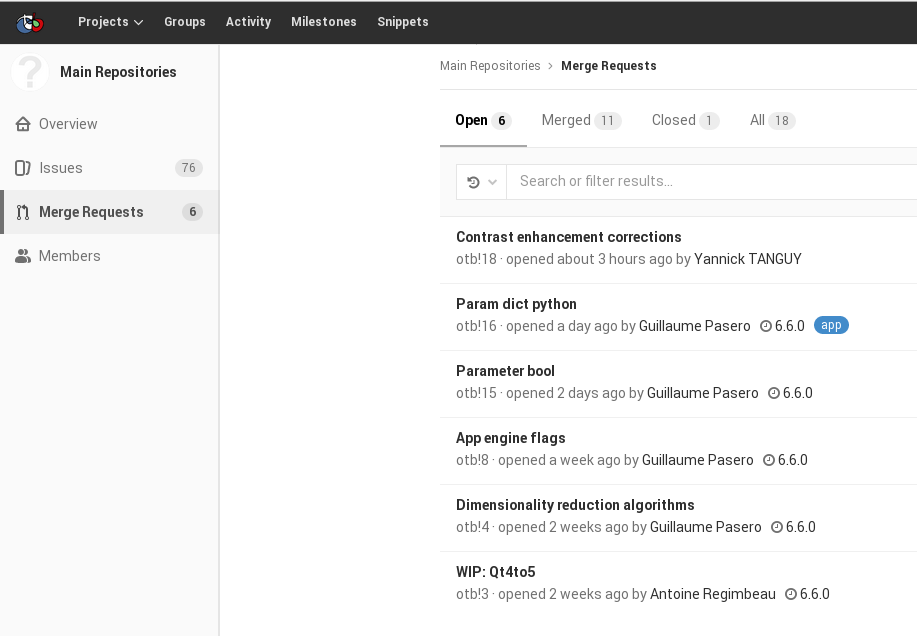
\includegraphics[width=\textwidth]{images/gitlab_mr.png}
    \end{columns}
\end{frame}


















\mode<all>
\section{Conclusion}
\begin{frame}
\frametitle{How many users?}
\begin{columns}[c]
\column{0.5\textwidth}
\begin{block}{Hard to tell\ldots}
\begin{itemize}
    \item $\approx$ 600 members on the otb-users list
    \item Between 100 and 150 mails by months
    \item $\approx$ 100 members on the developers list
    \item $\approx$ 118 user accounts on the bug tracker
    \item $\approx$ 50 contributors in the documentation
    \item $\approx$ 3400 downloads for OTB 5.0 on SourceForge(released June 1, 2015).
  \end{itemize}
\end{block}
\begin{block}{2015, 2016 and 2017 Users Days}
  15 to 20 atendants in Toulouse during 3 days
\end{block}
\column{0.5\textwidth}
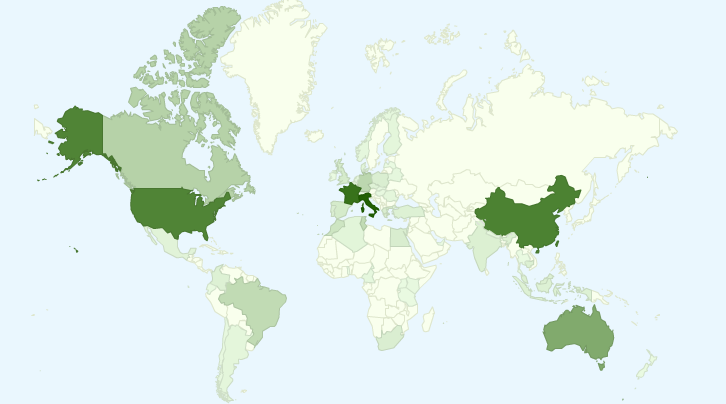
\includegraphics[width=0.9\textwidth]{images/OTB4_download_sourceforge_country_crop.png}\\
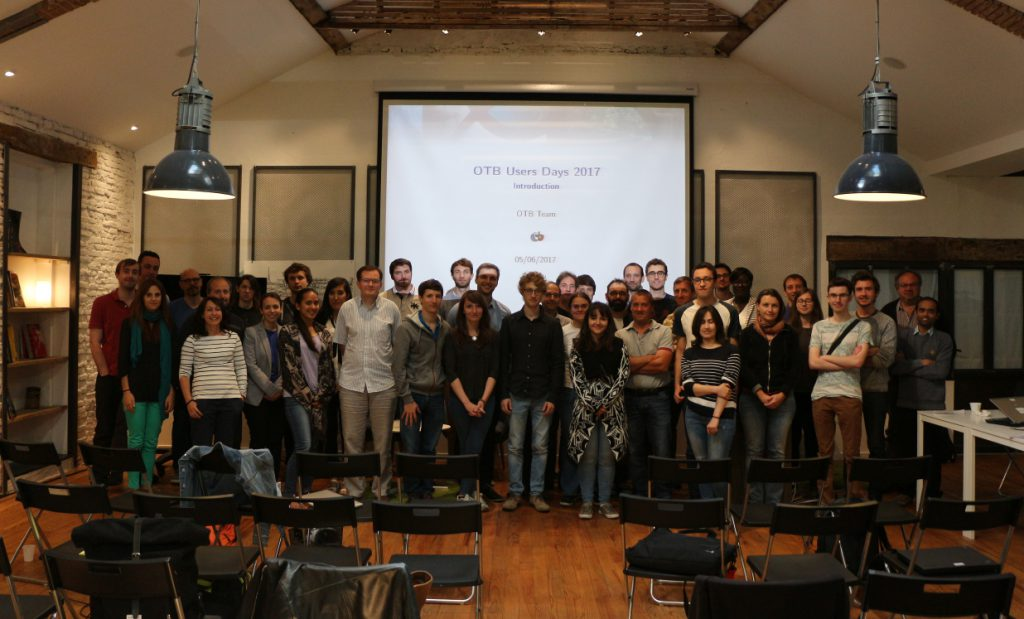
\includegraphics[width=0.9\textwidth]{images/userdays2017.jpg}
\end{columns}
\end{frame}

\begin{frame}
  \frametitle{Success stories}
  \vspace{-0.5cm}
\begin{columns}
\column{0.65\textwidth}
\begin{itemize}
\item OTB has been useful to ORFEO users and has processed 619 Pléiades
  images on RTU web site
\item Several training courses (3/5-day courses) given in France, Belgium,
Madagascar, UNESCO, Hawaii,Finland\ldots
\item OTB provides many useful RS functions in \textbf{one single tool}
\item OTB helped to improve the open-source codec for JP2 OpenJpeg
\item OTB equals or beats state-of-the-art tools (open source and maybe \$\$) on some points:
  \begin{itemize}
  \item band calculator
  \item tile-wise segmentation of full imagery
  \item full scene classification with a range of machine learning algorithms
  \item bridges between RS and GIS \ldots
  \end{itemize}
\item Beyond Orfeo, OTB is already used in several projects and software
\item OSGeo graduation
\end{itemize}
\column{0.35\textwidth}
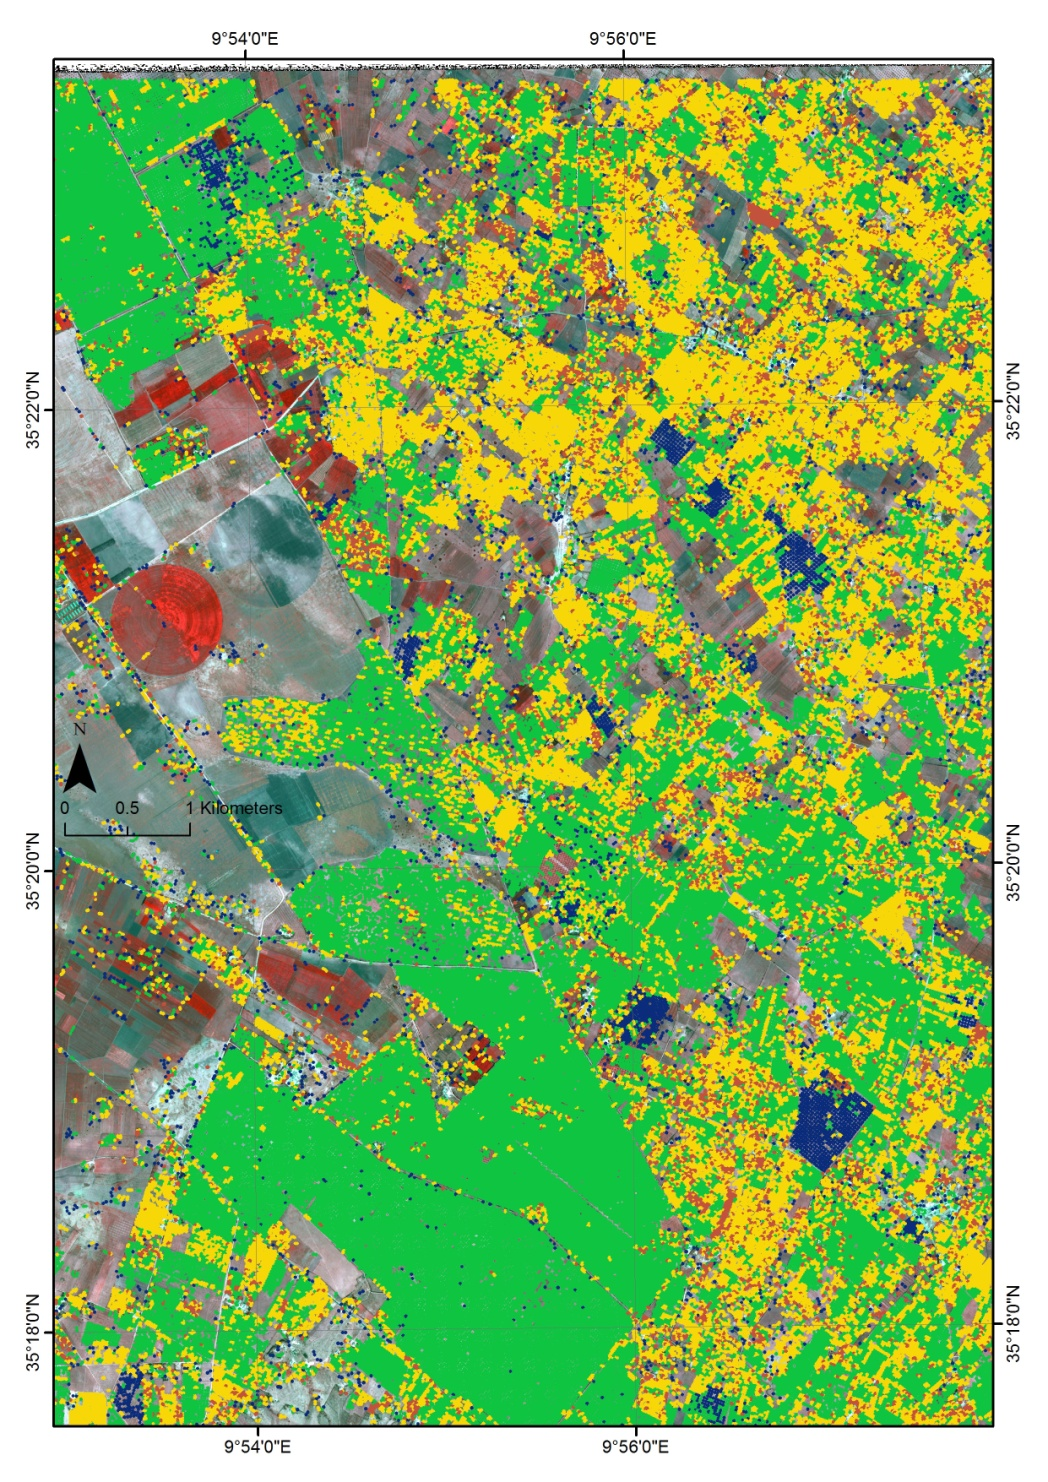
\includegraphics[width=0.9\textwidth]{images/resultats_ird.png}\\
\tiny{Thematic map from OTB segmentation, B. Mougenot~-~IRD}
\end{columns}
\end{frame}

\begin{frame}
  \frametitle{Projects and software using OTB}
  \vspace{-0.5cm}
\begin{columns}
  \column{0.55\textwidth}
  \begin{itemize}
    \item OTB applications are available in QGIS and in Zoo Project (WPS service)
    \item OTB is a component of \alert{Sentinel-2} and Venus ground segment (CNES and ESA)
    \item Terr'Image: Educational software for satellite image analysis
    \item Use to prototype \alert{THEIA} products from the Scientific Expertise Centres
    \item ESA Sentinel-2 for Agriculture
    \item Gnorasi Software (National Technical University of Athens)
    \item Geosud project(IRSTEA)
    \item TCM research program (ETS Quebec)
    \item Processing chains at CEREMA and SERTIT
  \end{itemize}
  \column{0.6\textwidth}
  \begin{center}
  \includegraphics[width=0.6\textwidth,height=0.35\textheight]{images/Carte_17Classes.png}\\
  \tiny{Prototype of THEIA Land cover product (CESBIO)}
  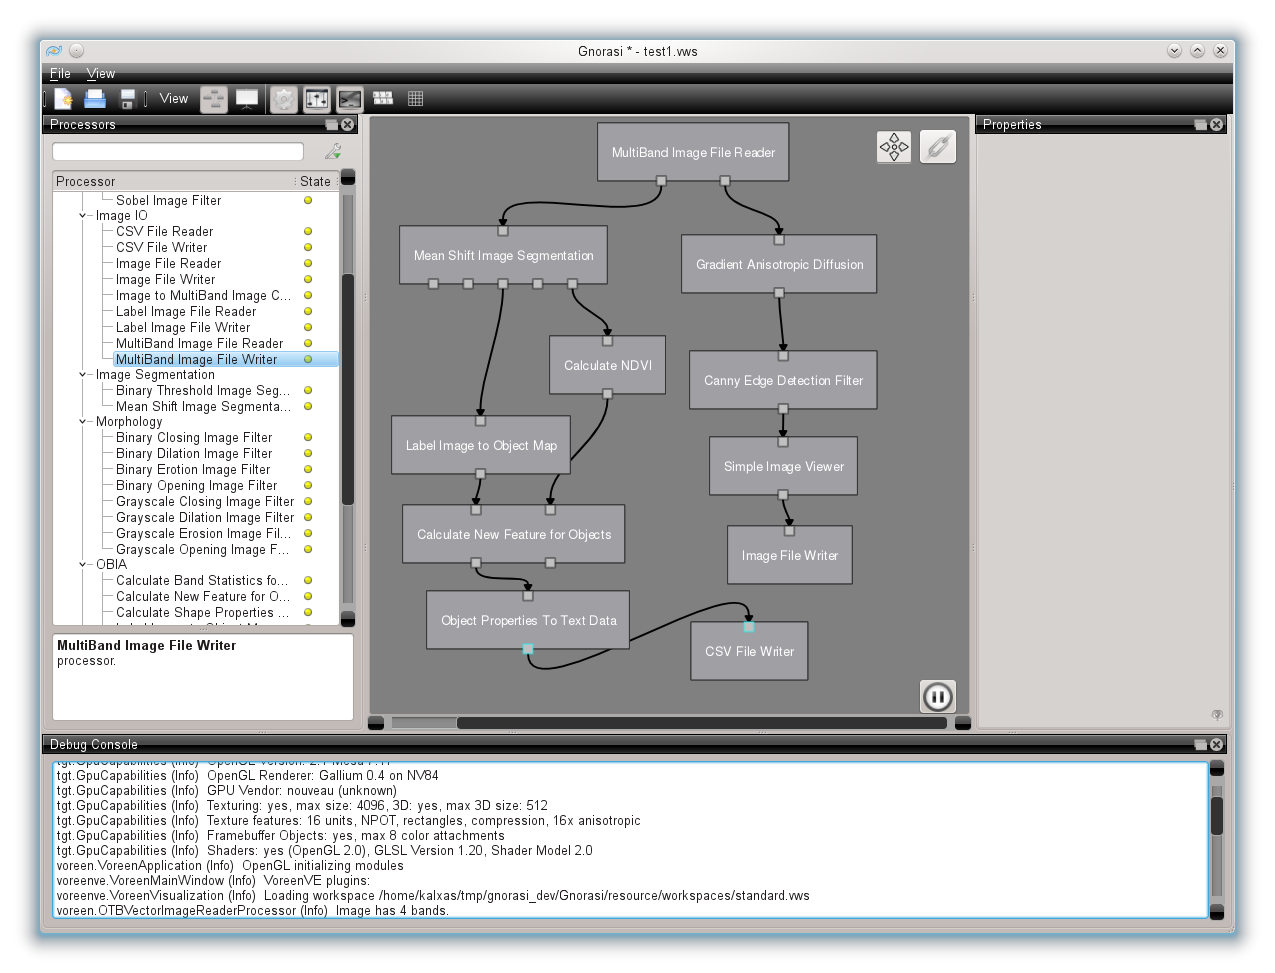
\includegraphics[width=0.6\textwidth,height=0.35\textheight]{images/gnorasi2.png}\\
  \tiny{The Gnorasi software}
  \end{center}
\end{columns}
\end{frame}

\begin{frame}
\frametitle{Support/Help/Contribute}
\vspace{-0.2cm}
\begin{block}{General resources}
\vspace{-0.2cm}
\begin{description}
\item[Site web] \href{http://www.orfeo-toolbox.org}{orfeo-toolbox.org}
\item[Wiki] \href{http://wiki.orfeo-toolbox.org}{wiki.orfeo-toolbox.org}
\item[Blog] \href{http://blog.orfeo-toolbox.org}{blog.orfeo-toolbox.org}
\end{description}
\end{block}
\vspace{-0.2cm}
\begin{block}{Documentation and help}
\vspace{-0.2cm}
\begin{description}
\item[Guides] Software Guide and CookBook (remote sensing recipes)
\item[Doxygen] \href{http://www.orfeo-toolbox.org/doxygen}{doxygen}
\item[Users mailing list] otb-users@googlegroups.com
\item[Developers mailing list] otb-developers@googlegroups.com
\end{description}
\end{block}
\vspace{-0.2cm}
\begin{block}{Follow-up}
\vspace{-0.2cm}
\begin{description}
\item[Look at the code?] \href{https://gitlab.orfeo-toolbox.org/orfeotoolbox/otb}{gitlab.orfeo-toolbox.org}
\item[Find a bug? Feature propositions?] \href{https://gitlab.orfeo-toolbox.org/orfeotoolbox/otb/issues}{gitlab.orfeo-toolbox.org/orfeotoolbox/otb/issues}
\item[Dashboard] \href{http://dash.orfeo-toolbox.org}{dash.orfeo-toolbox.org}
\end{description}
\end{block}
\end{frame}

\begin{frame}
\frametitle{Thank you! Any questions?}
\begin{minipage}[t][6cm][t]{\textwidth}
\begin{center}
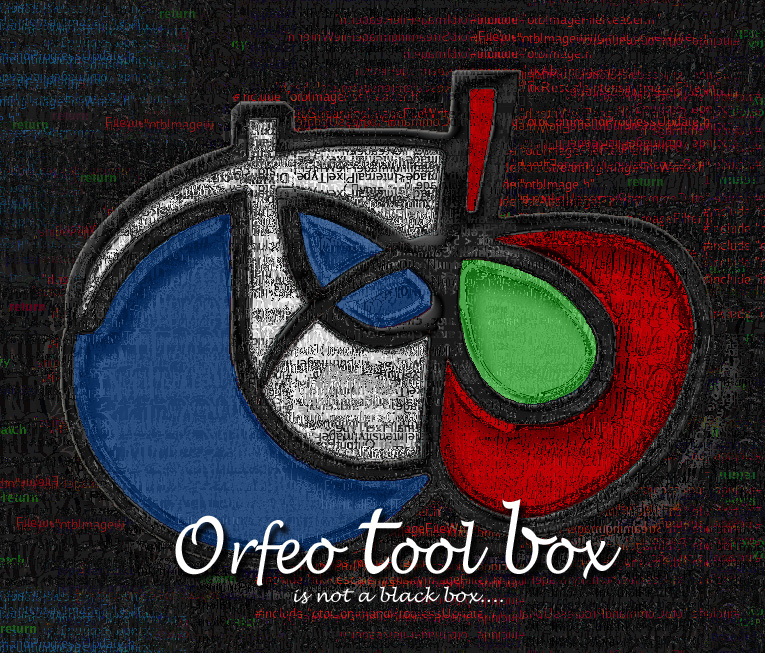
\includegraphics[width=0.65\textwidth]{images/LOGOTB_blackbox.png}
\end{center}
\end{minipage}
\end{frame}


\end{document}
